% výběr
Na internetu se dá najít spoustu cloudových řešení, které bych mohl využít. Řešení z nichž některá byla přímo vytvořená 
pro sběr a zobrazení dat z chytrých senzorů, se mi úplně nelíbila. Důvodů bylo několik. Řešení vytvořená \uv{na míru} 
měla zásadní problém v tom, že většinou v tarifu zdarma měla nějaké významné omezení, například omezení ukládaných dat 
pouze na poslední tři měsíce a platit se mi nechtělo(\url{https://io.adafruit.com/}). Z ostatních jsem vybral 
\gls{firebase}, poněvadž měl rozumně nastavené limity zdarma, nádhernou dokumentaci a zároveň za ním stojí velká firma, 
takže se nemusím bát, že za rok skončí(\url{https://firebase.google.com/pricing}).

\subsection{Firebase}
% založení
\gls{firebase} je služba Googlu, takže jediné co je potřeba pro založení je Google účet, díky tarifu zdarma ani nechce 
žádnou platební kartu. Založení projektu se pokusím osvětlit několika obrázky. Počáteční adresa je 
\url{https://console.firebase.google.com/u/0/}

% krok 1
\begin{figure}[H]
    \centering
    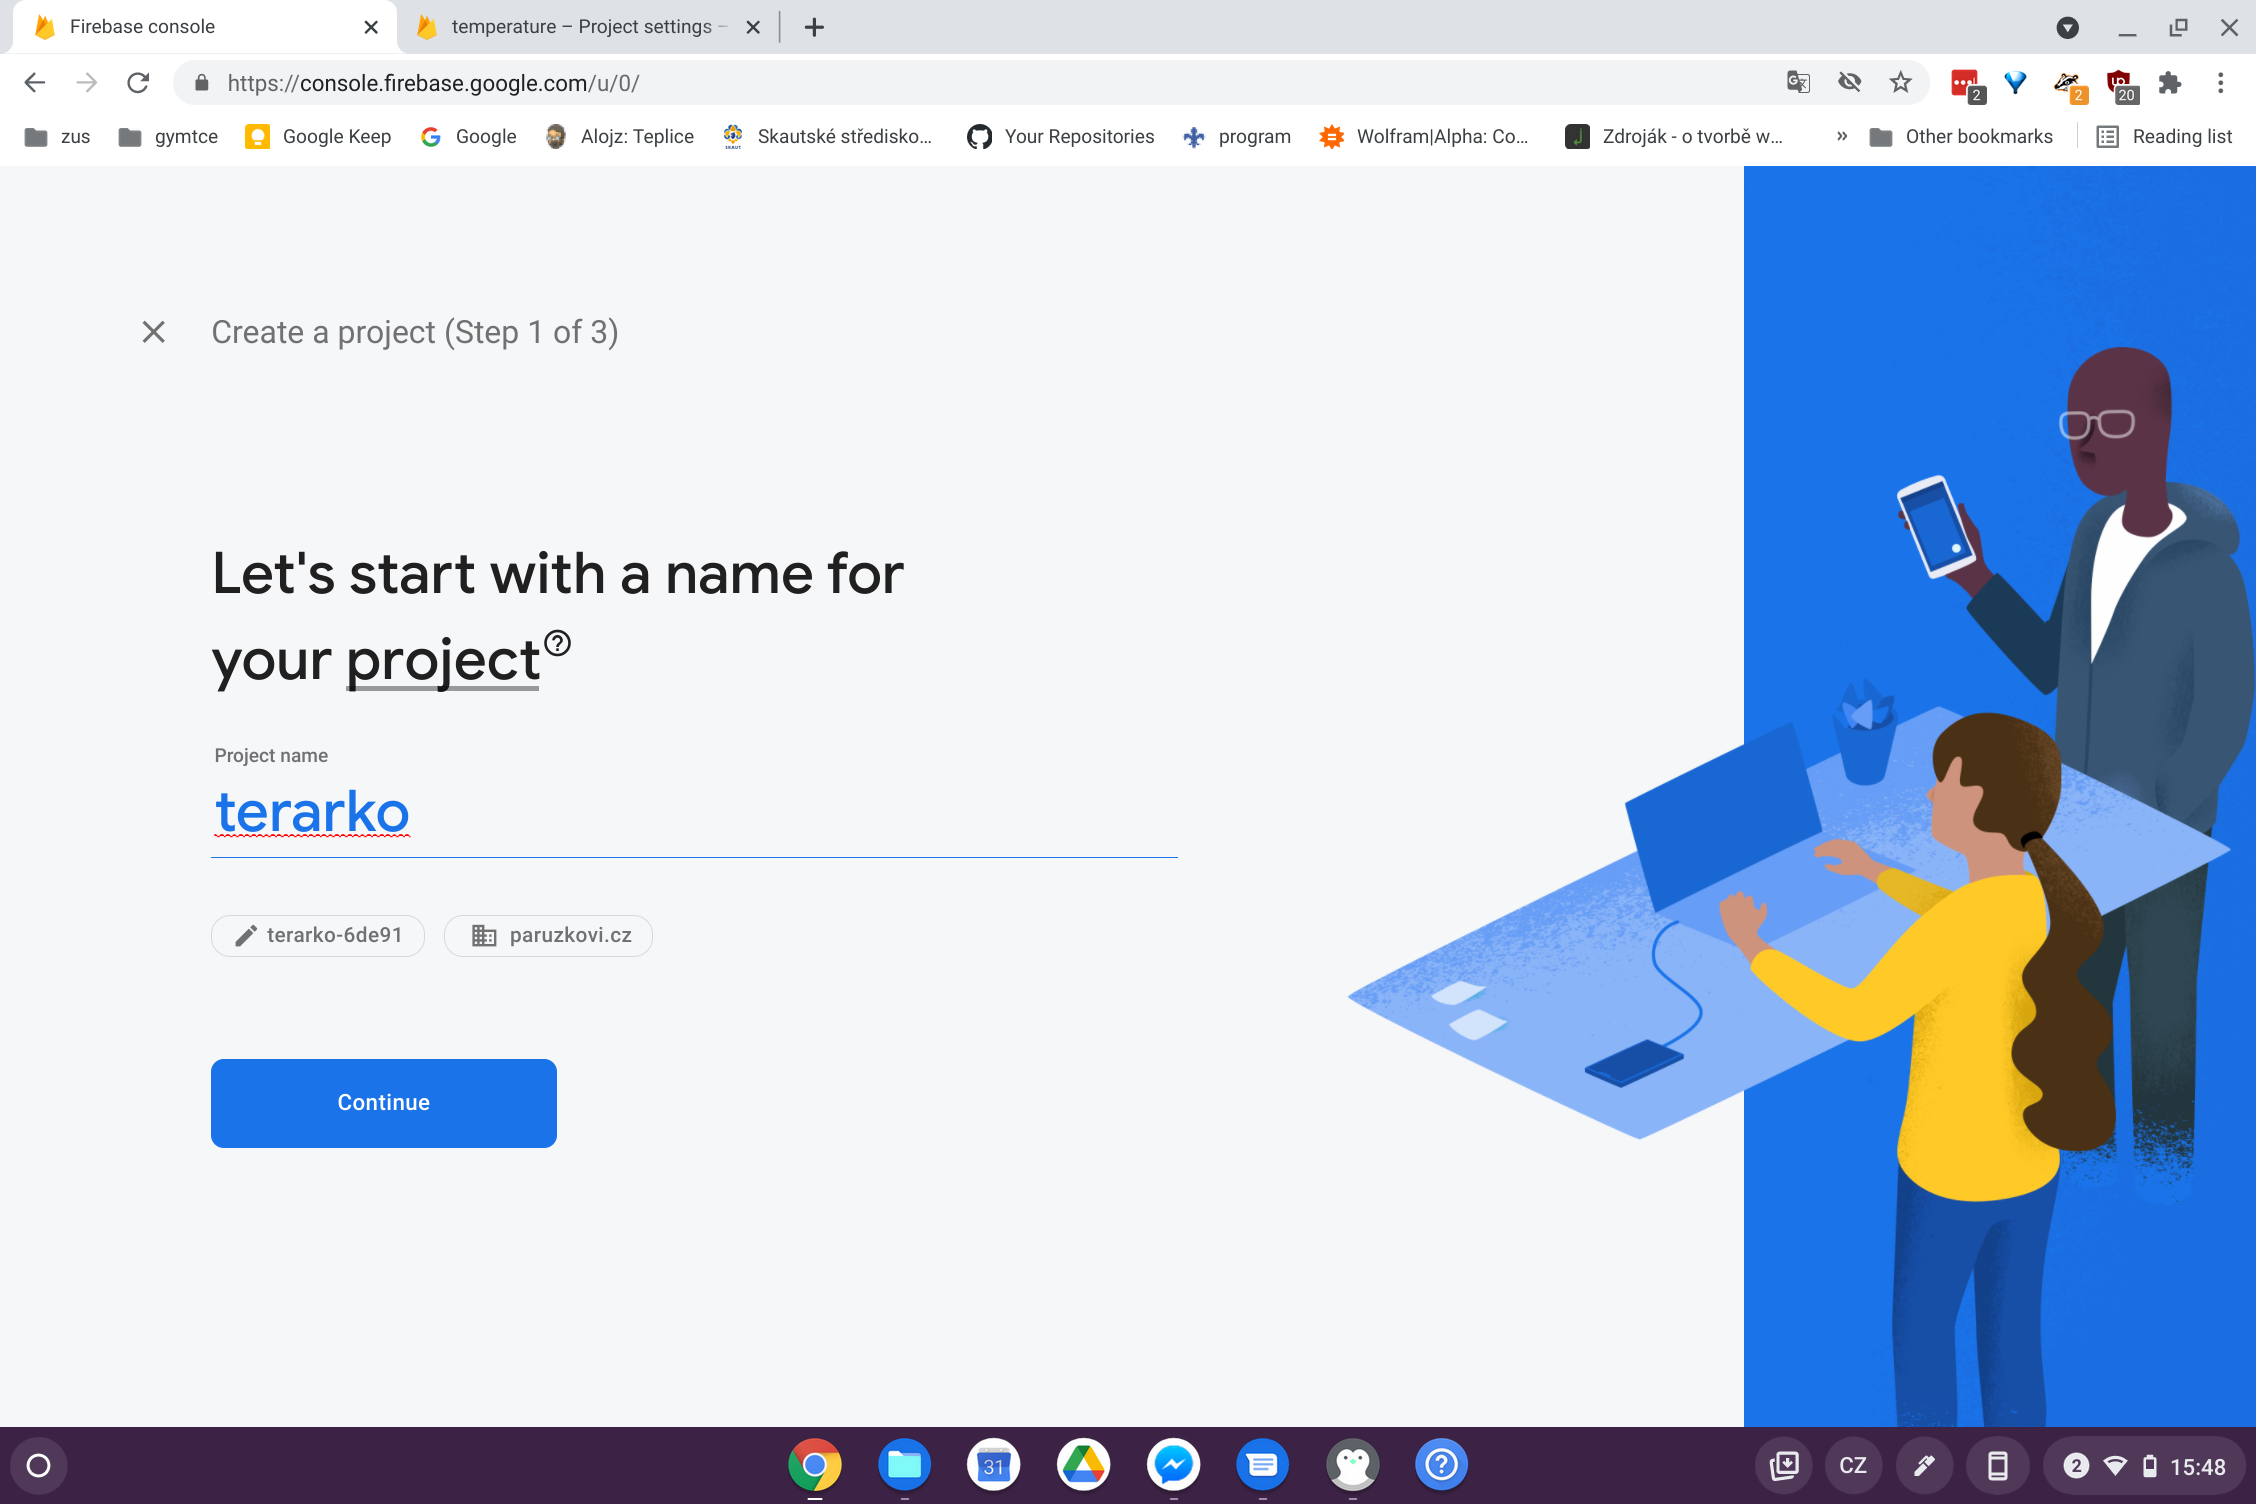
\includegraphics[width=0.8\textwidth]{firebase-1.png}
    \caption{Firebase, krok 1}
\end{figure}
V kroku 1 vybírám projektu jméno.
%krok 2
\begin{figure}[H]
    \centering
    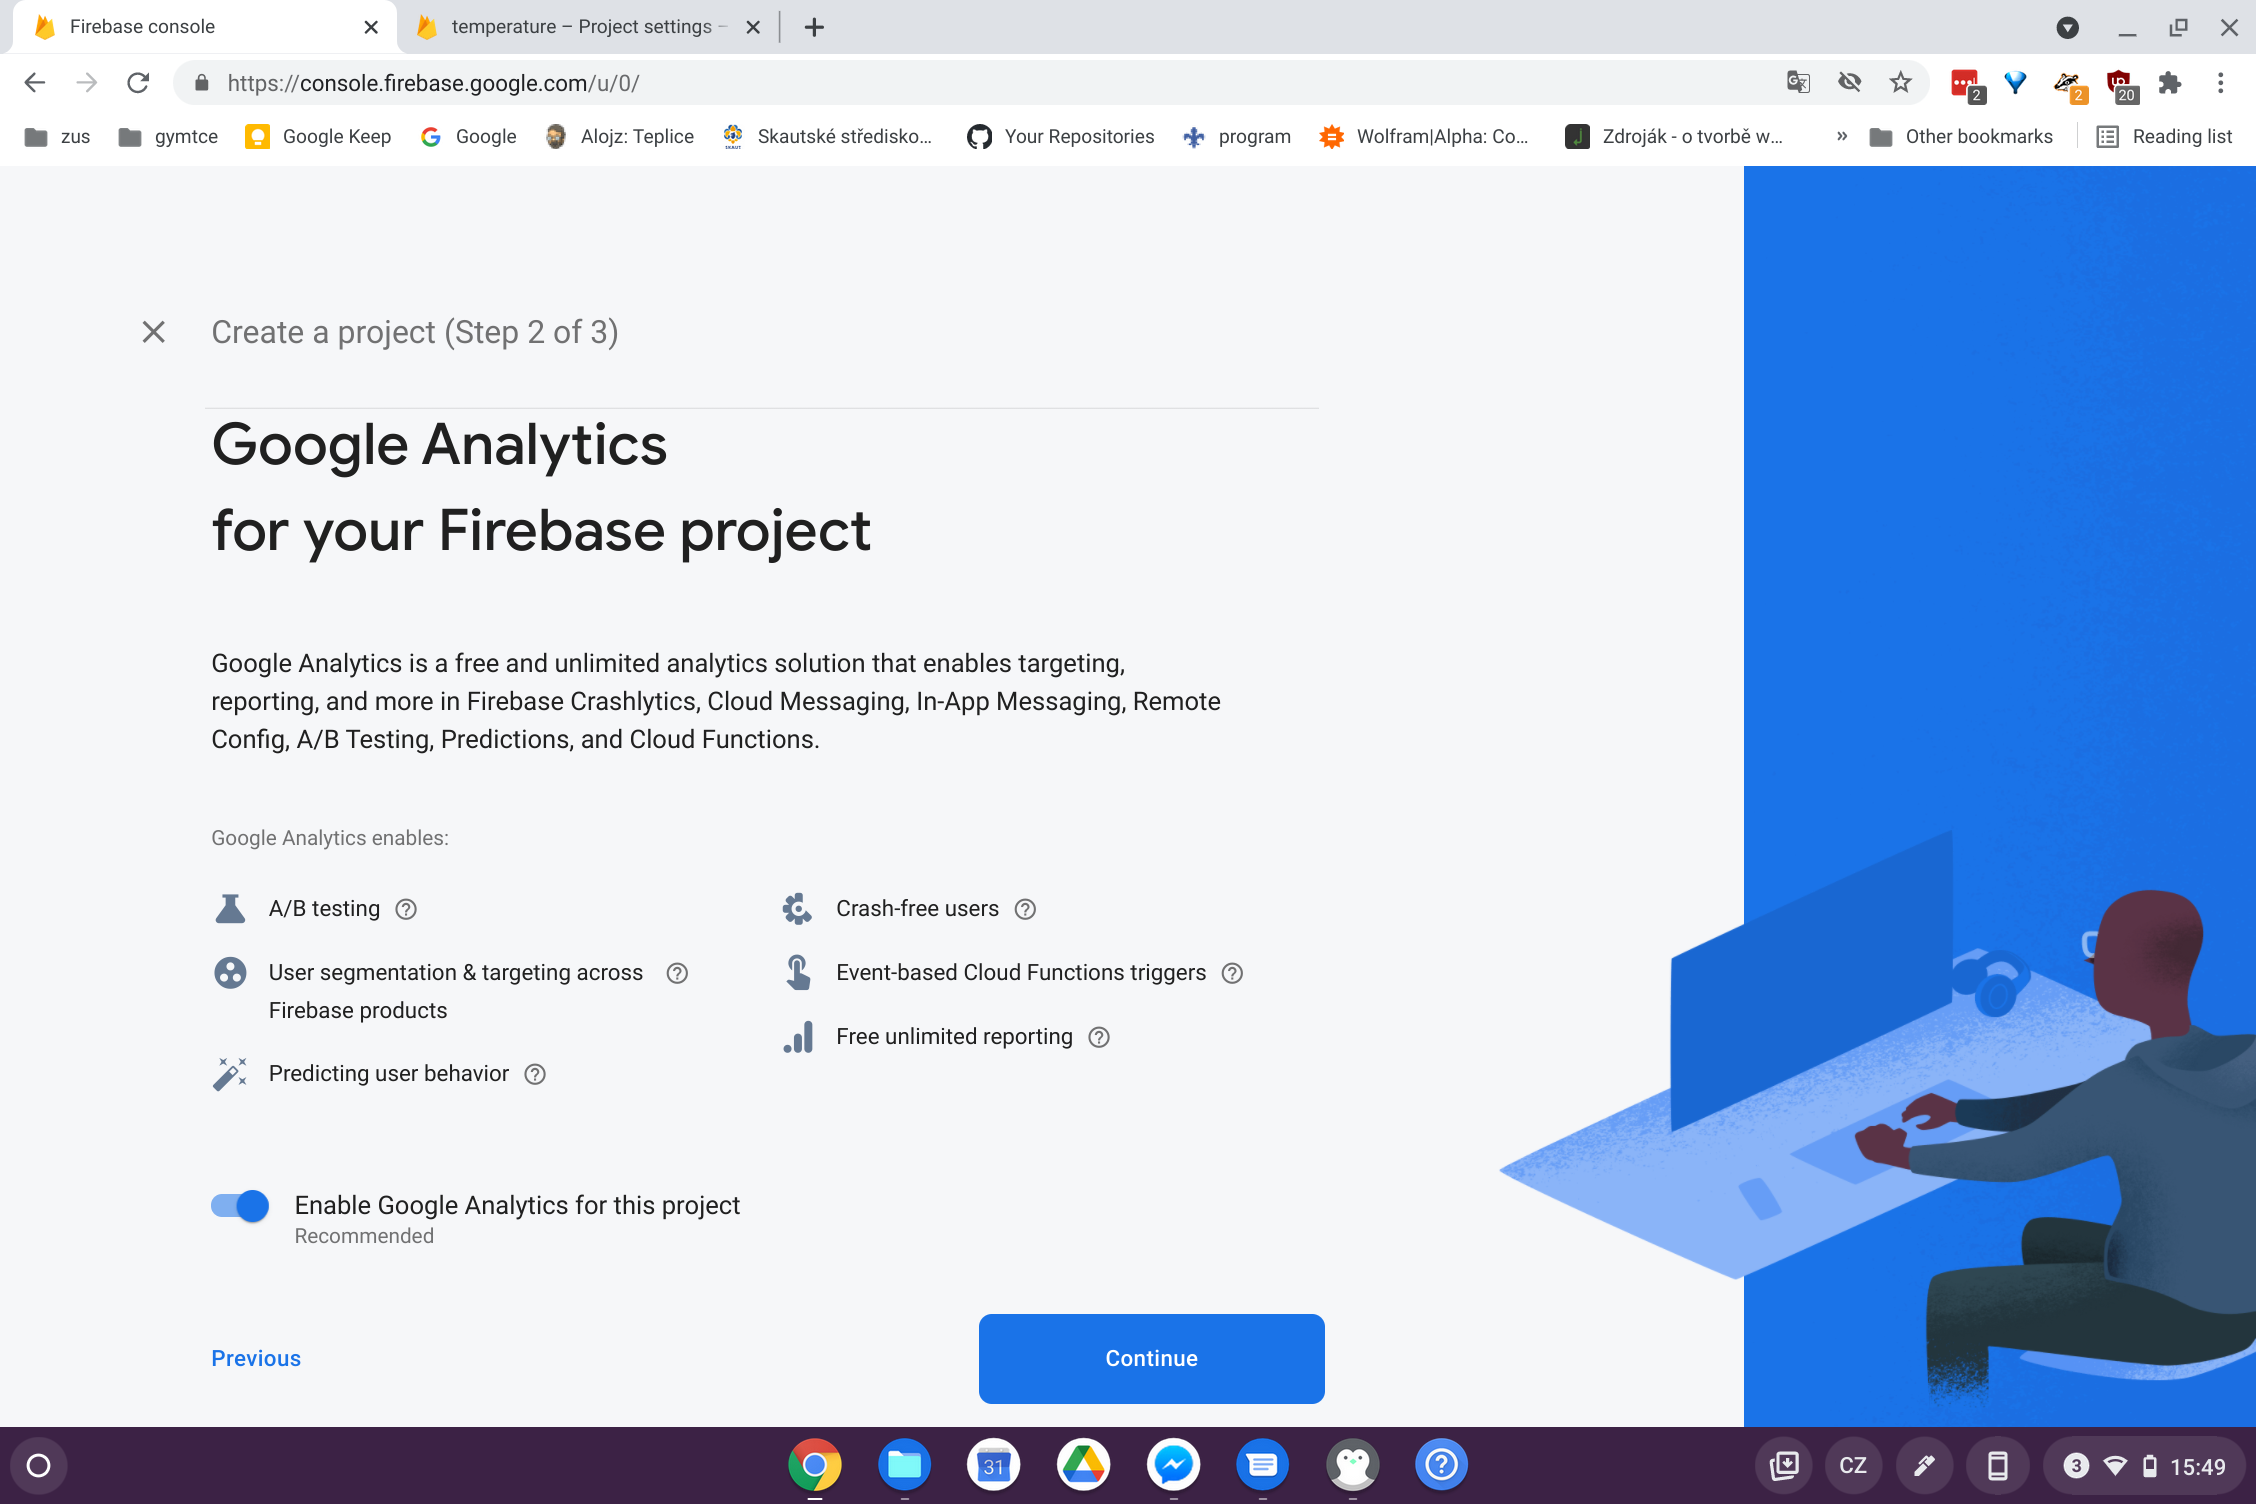
\includegraphics[width=0.8\textwidth]{firebase-2.png}
    \caption{Firebase, krok 2}
\end{figure}
V kroku 2 můžu pro projekt povolit Google Analytics.
% krok 3
\begin{figure}[H]
    \centering
    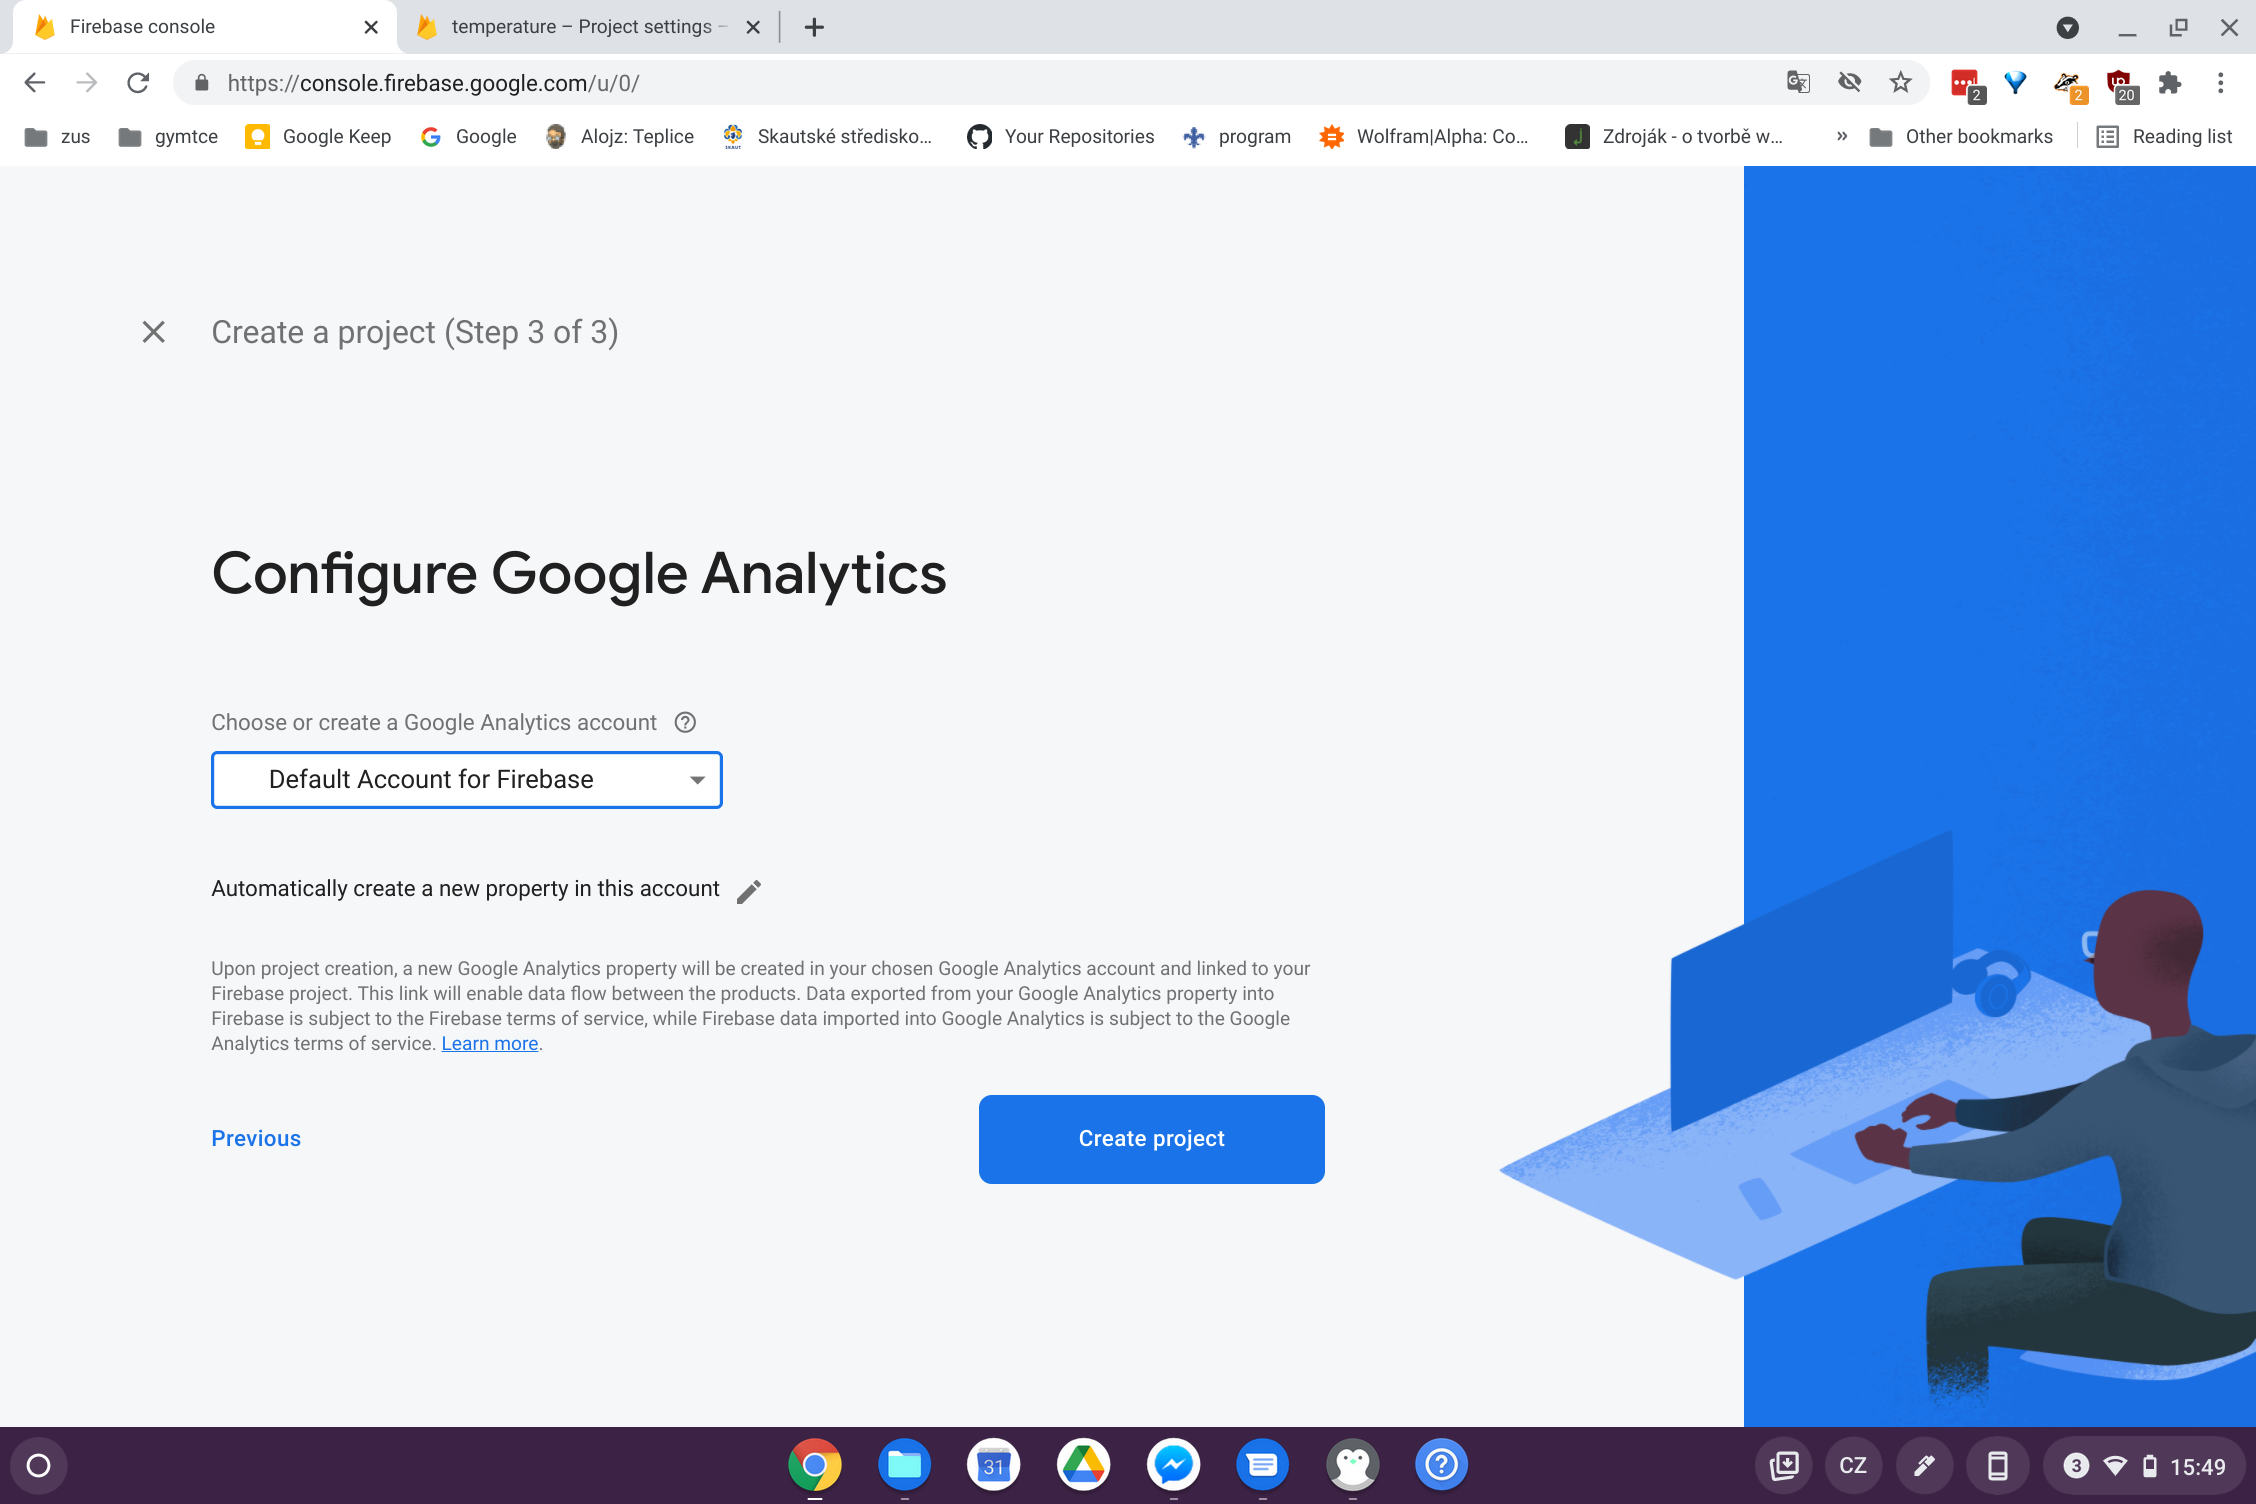
\includegraphics[width=0.8\textwidth]{firebase-3.png}
    \caption{Firebase, krok 3}
\end{figure}
V kroku 3 přiřazuji účet Google Analytics.% hotovo
\begin{figure}[H]
    \centering
    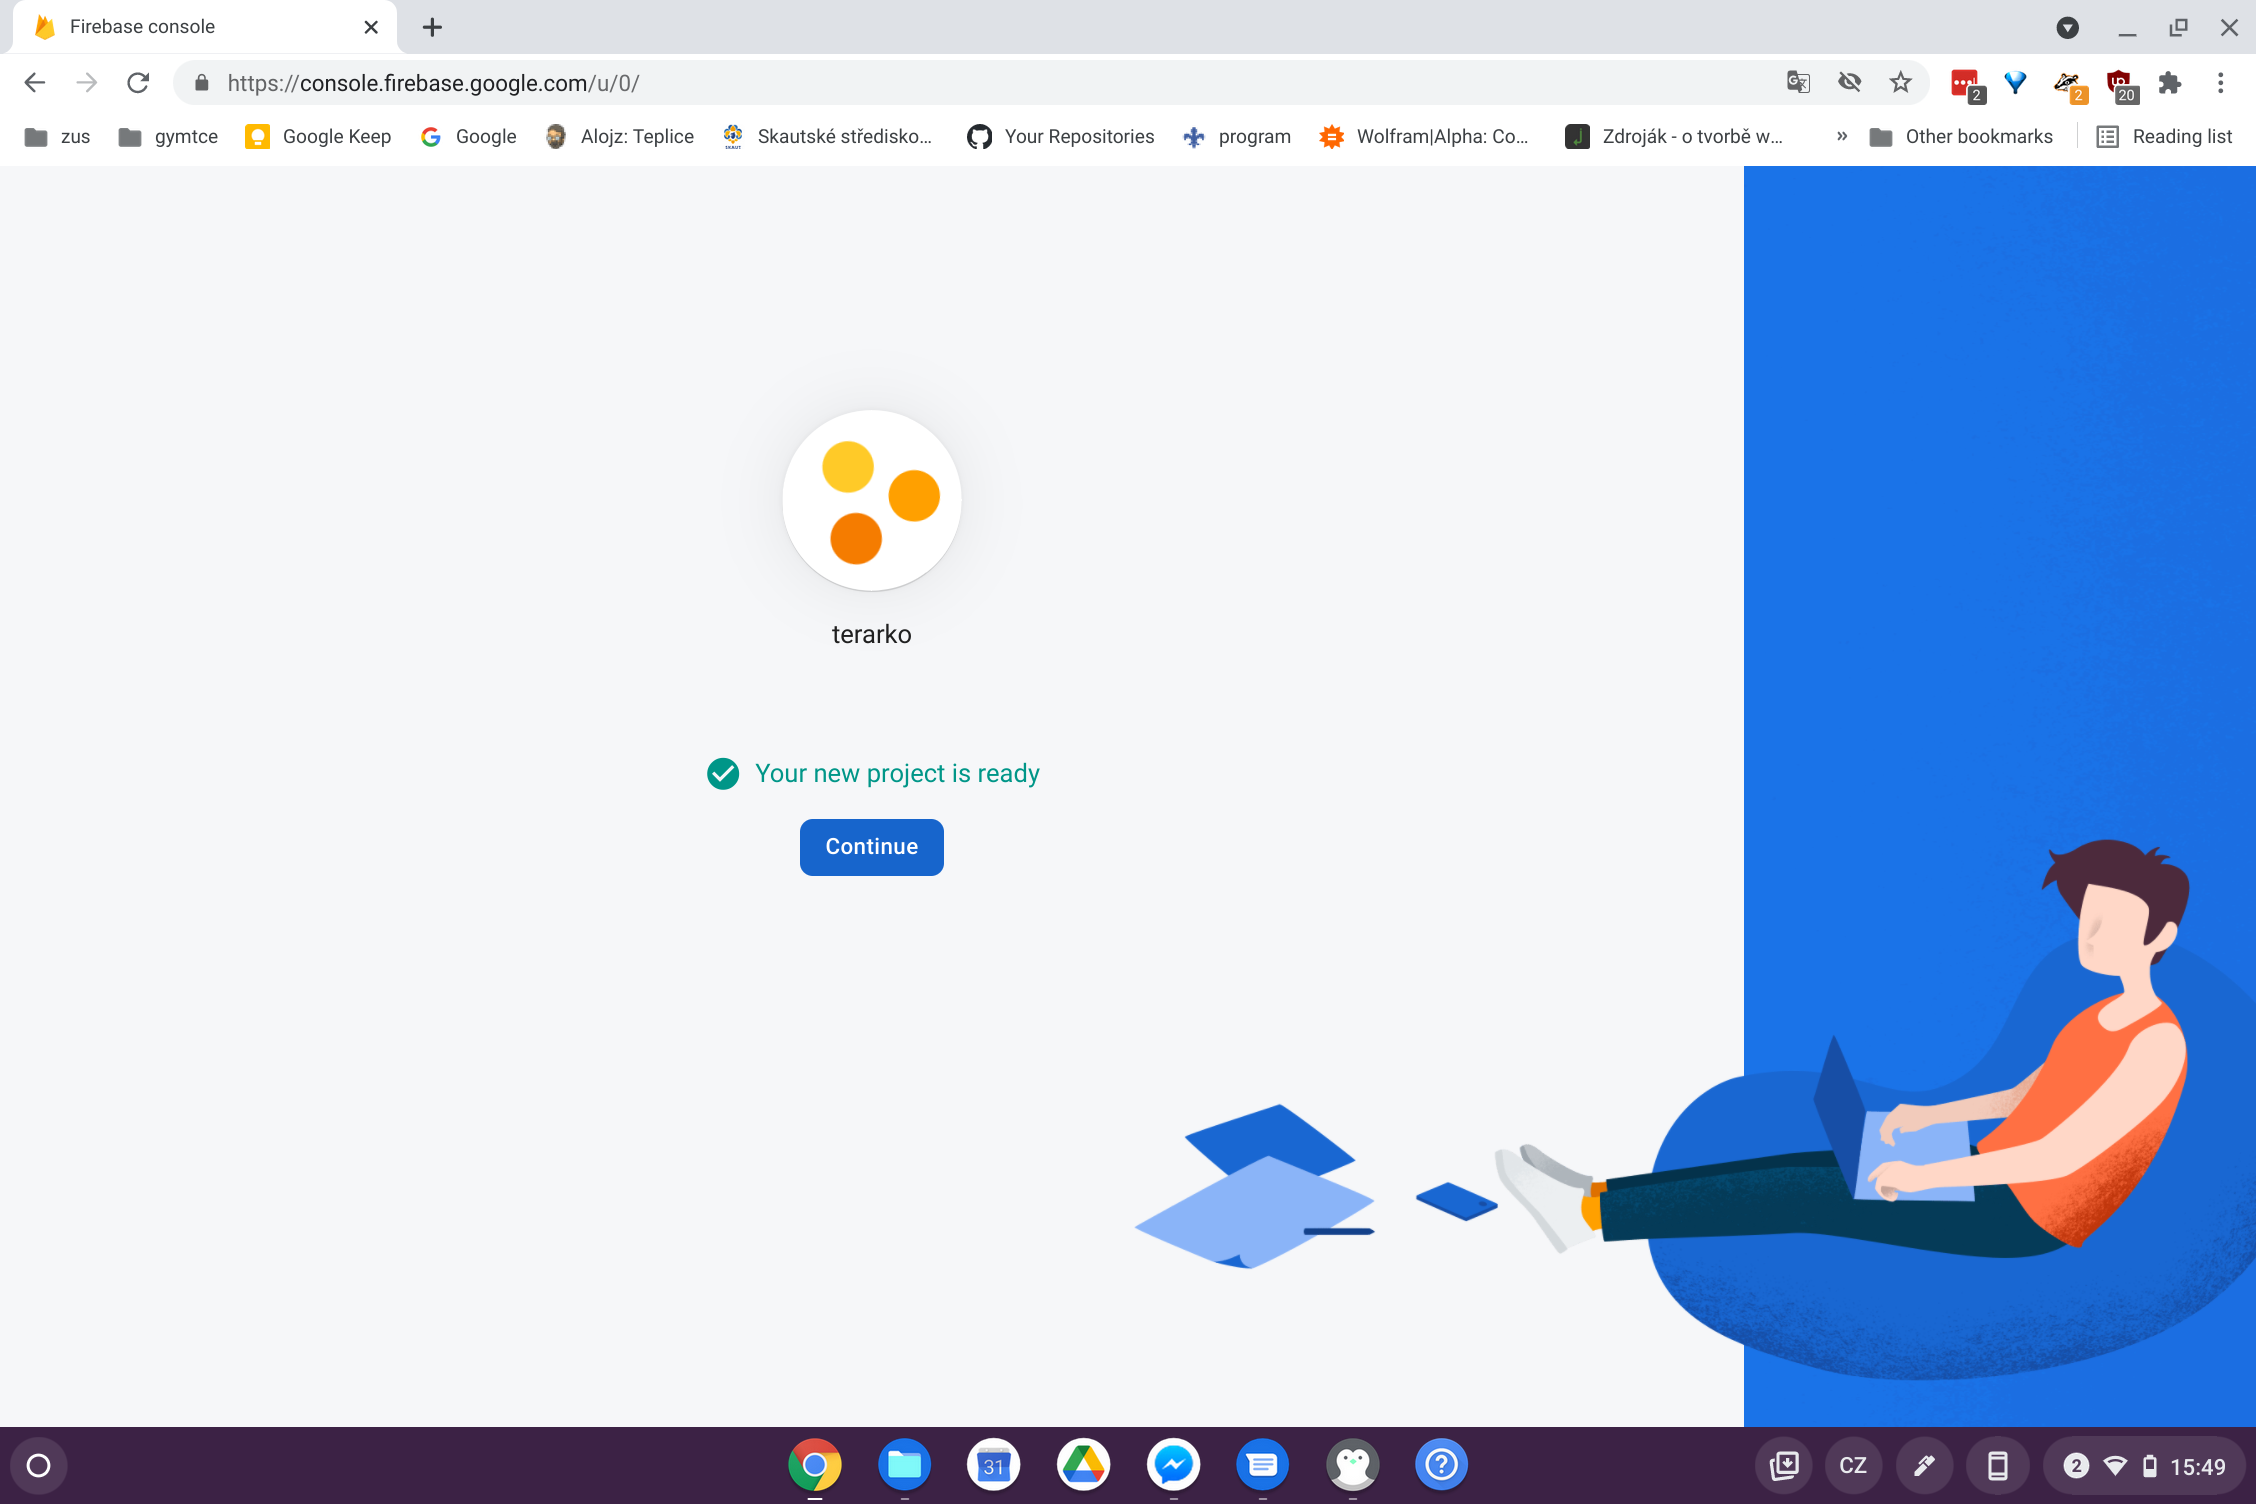
\includegraphics[width=0.8\textwidth]{firebase-fin.png}
    \caption{Firebase, hotovo}
\end{figure}
Vše jsem ponechal na výchozích hodnotách, teoreticky bych vzhledem k účelu mohl vypnout Google Analytics.
% dashboard
\begin{figure}[H]
    \centering
    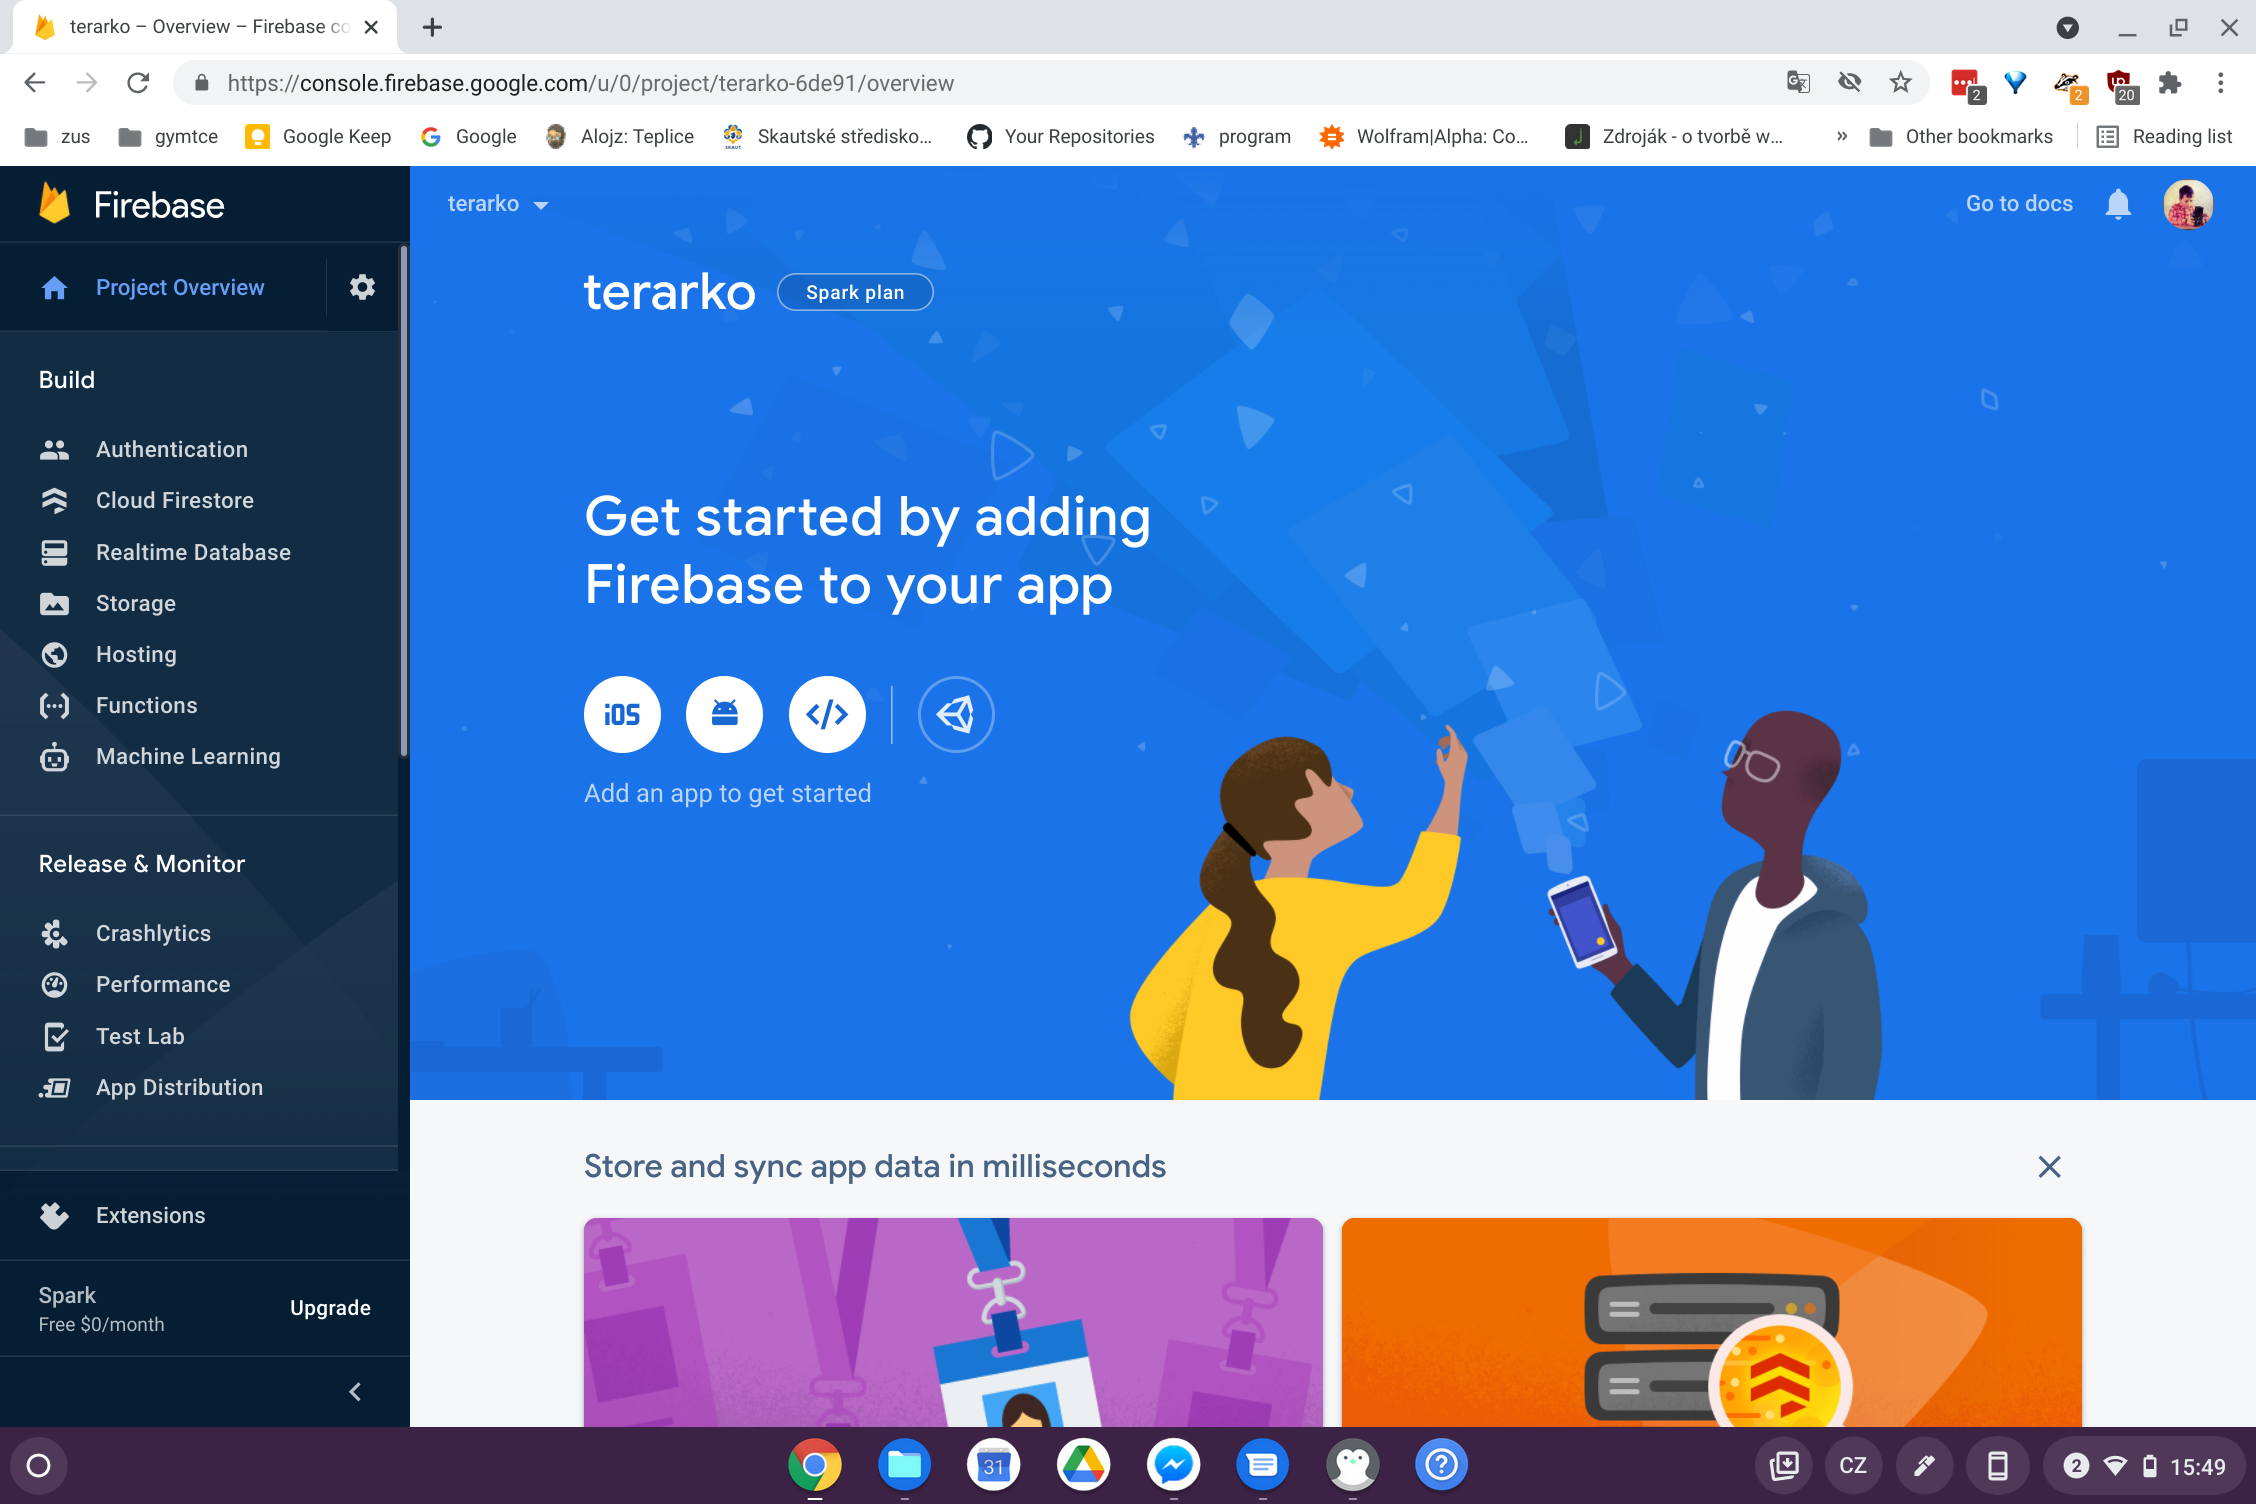
\includegraphics[width=0.8\textwidth]{firebase-dashboard.png}
    \caption{Firebase}
\end{figure}
Takto vypadá úvodní stránka \gls{firebase} po založení. Teď můžu přidat aplikace, které budu používat.

\subsection{Firestore}
Jako první přidám firestore, což je rychlá \gls{nosql} databáze, kterou budu používat pro ukládání naměřených hodnot. 
Opět se pokusím vysvětlit několika obrázky.

% krok 1
\begin{figure}[H]
    \centering
    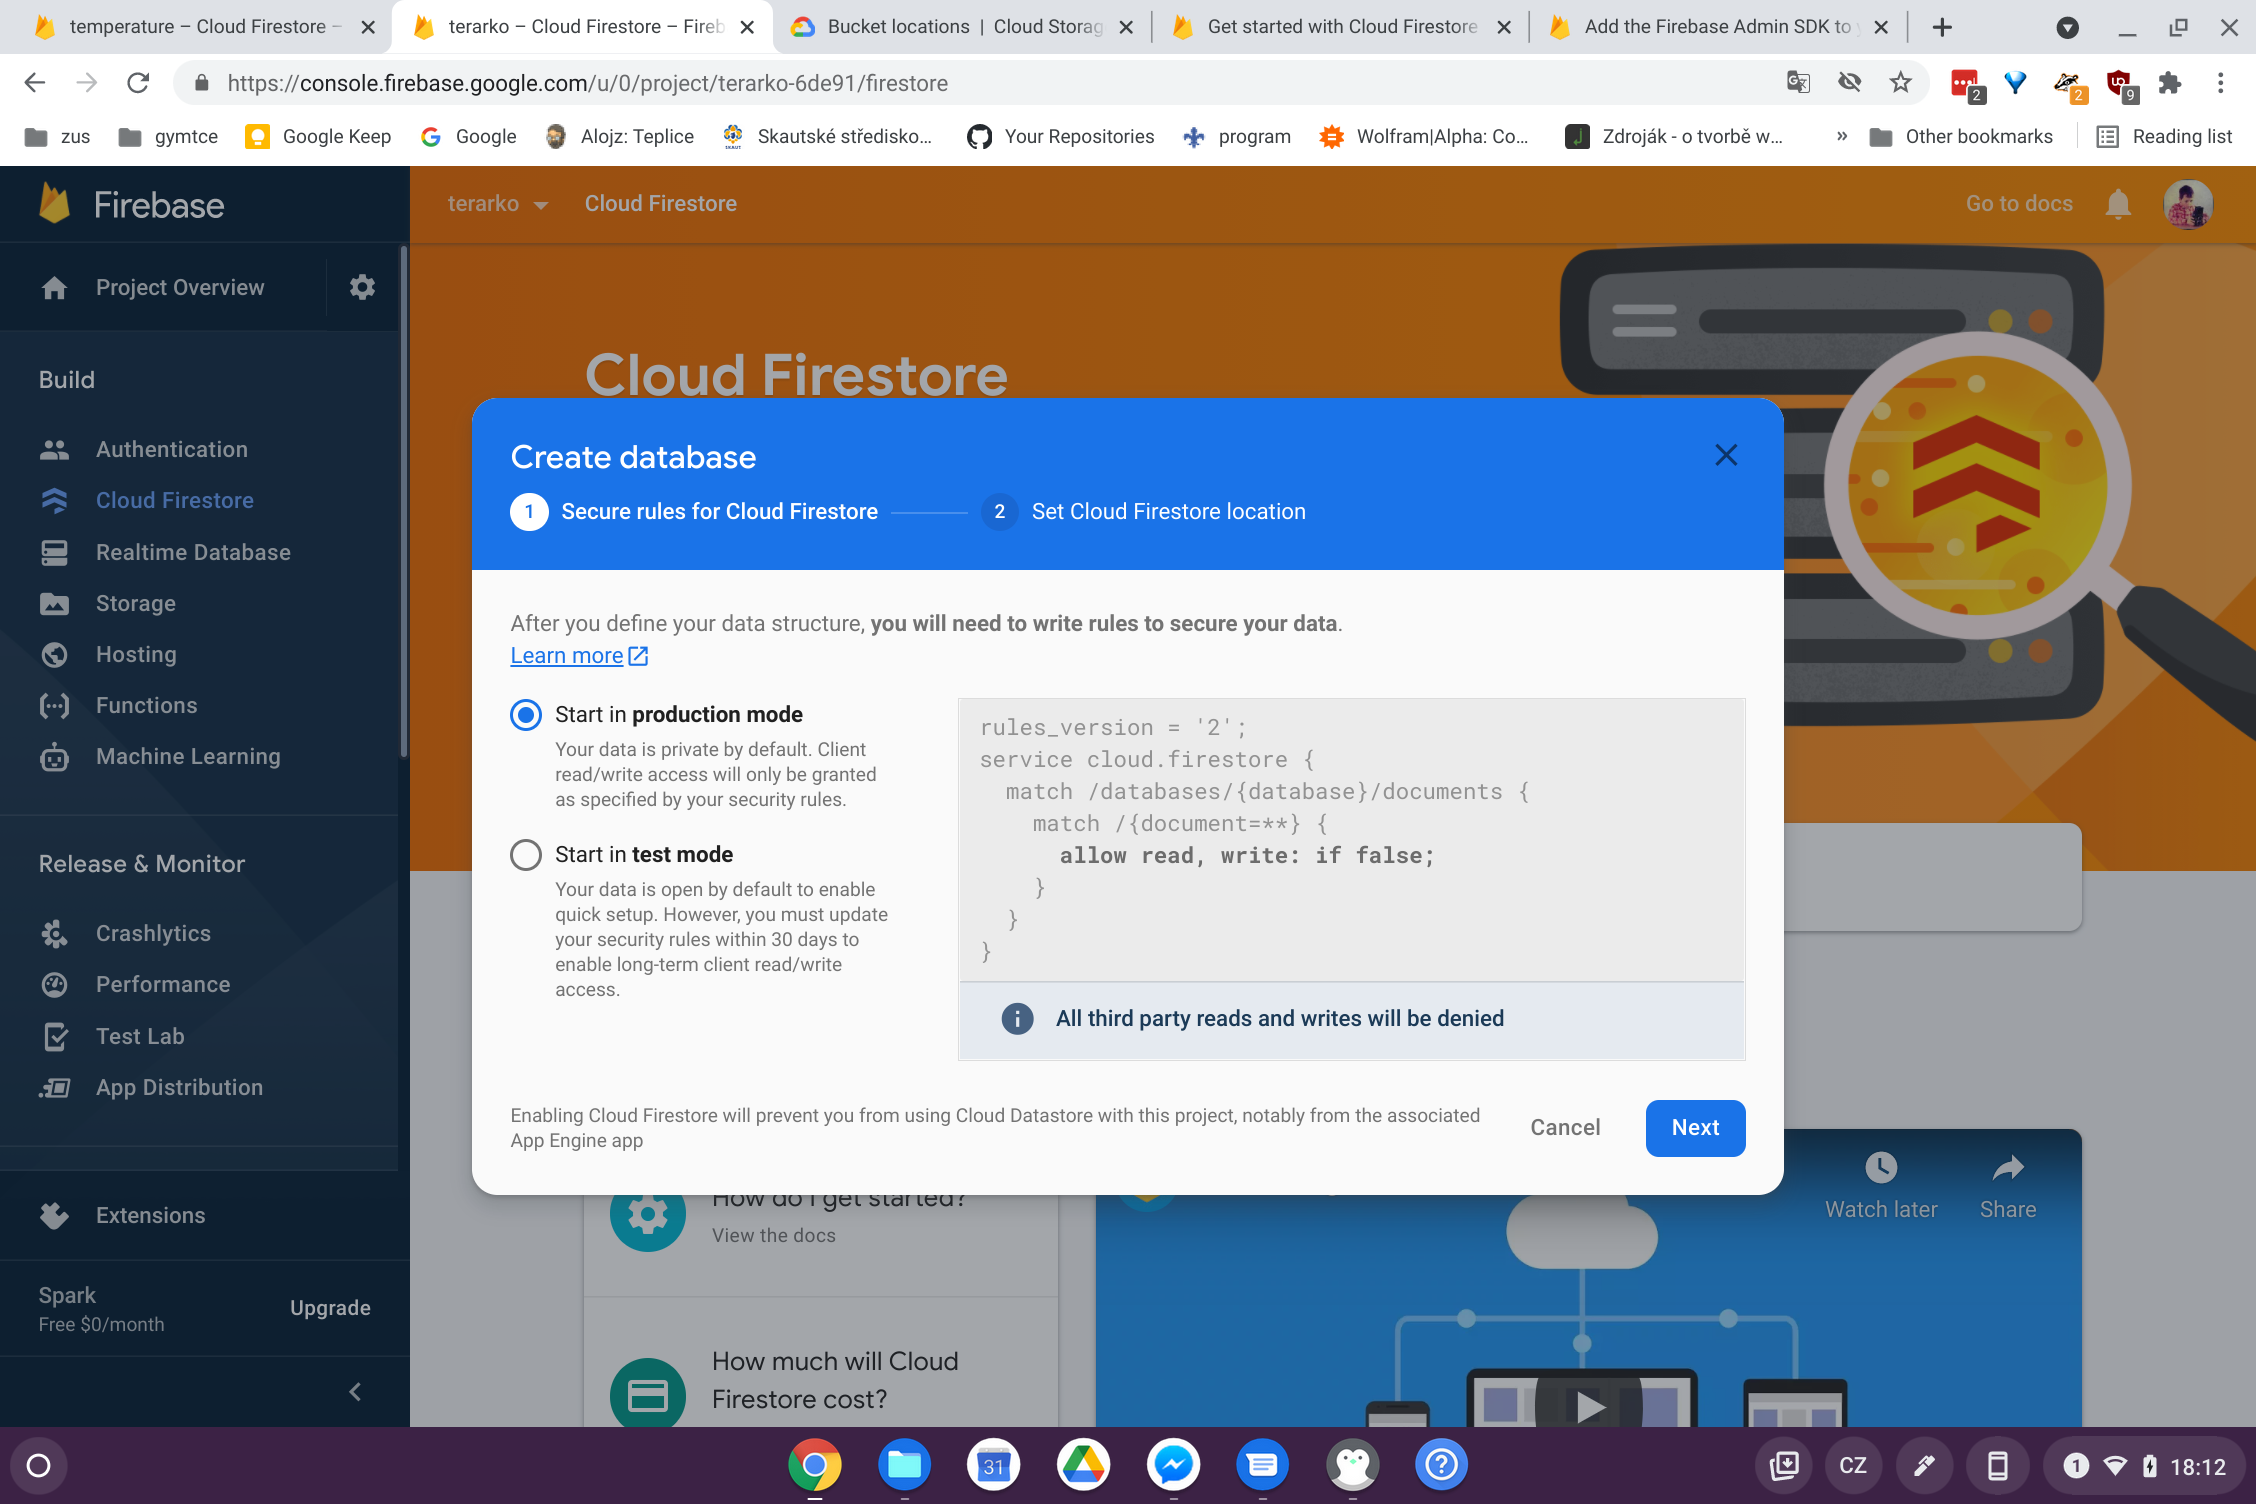
\includegraphics[width=0.8\textwidth]{firestore-1.png}
    \caption{Firestore, krok 1}
\end{figure}
Nastavení bezpečnosti použiji v produkčním módu, nechci aby se mi tam někdo připojoval bez přihlášení.
% krok 2
\begin{figure}[H]
    \centering
    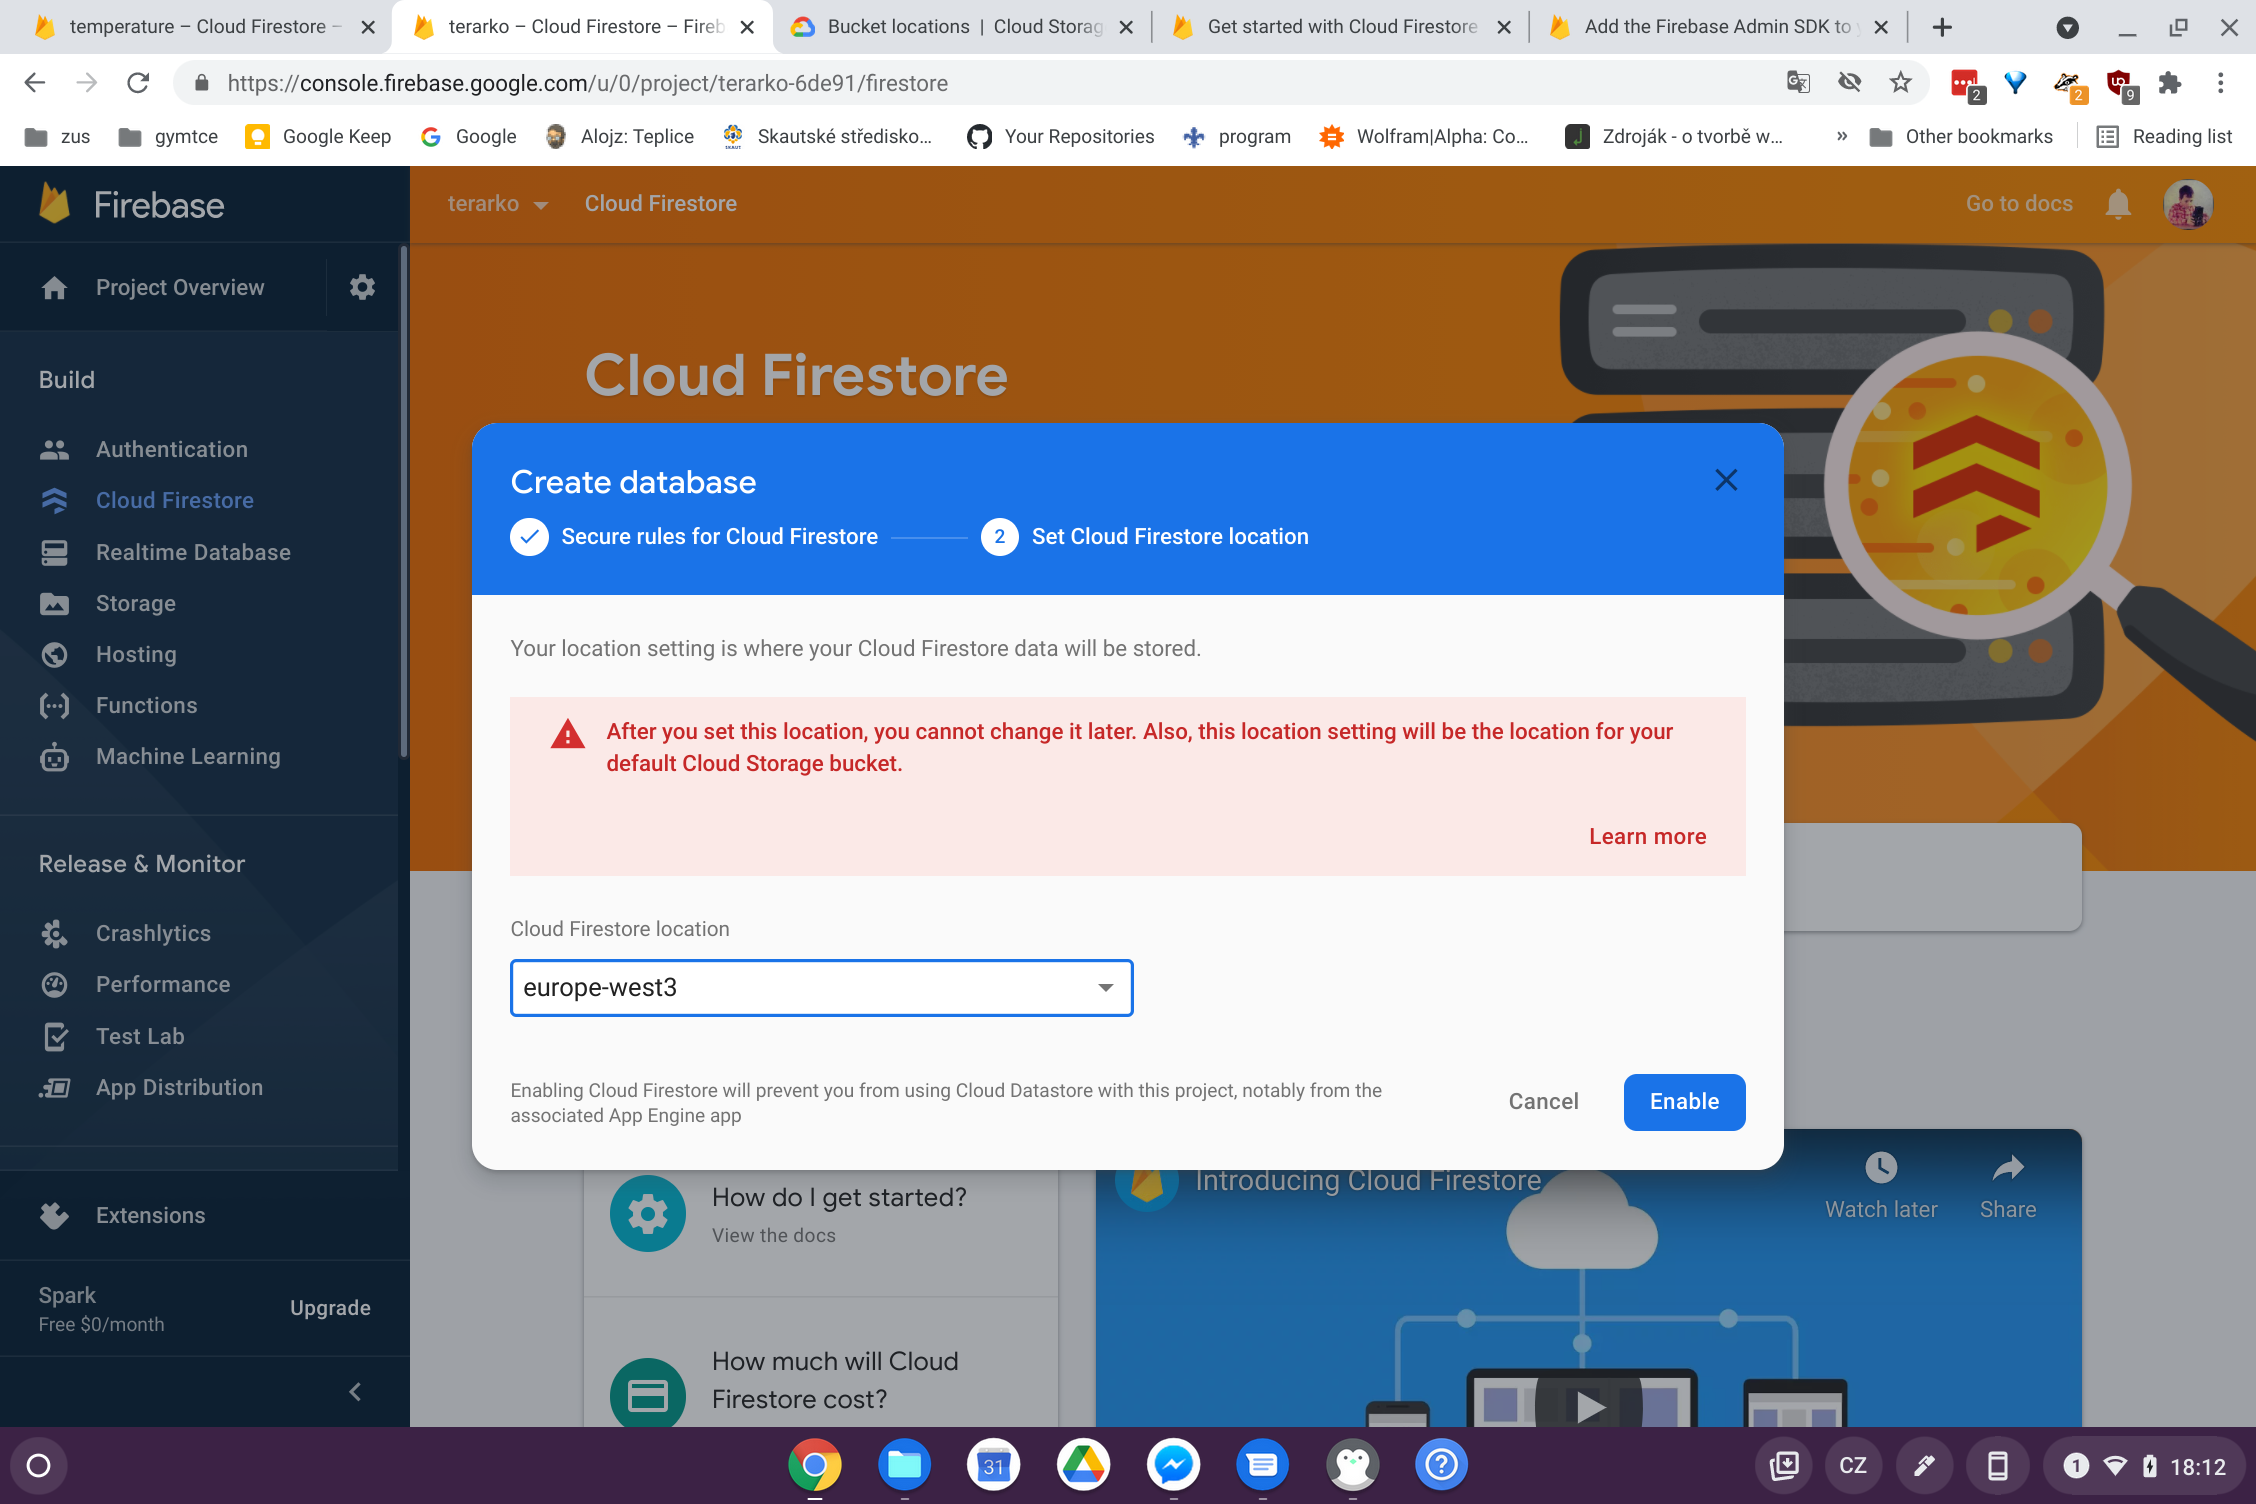
\includegraphics[width=0.8\textwidth]{firestore-2.png}
    \caption{Firestore, krok 2}
\end{figure}
Jako lokaci databáze volím Evropu konkrétně Frankfurt.
% dashboard
\begin{figure}[H]
    \centering
    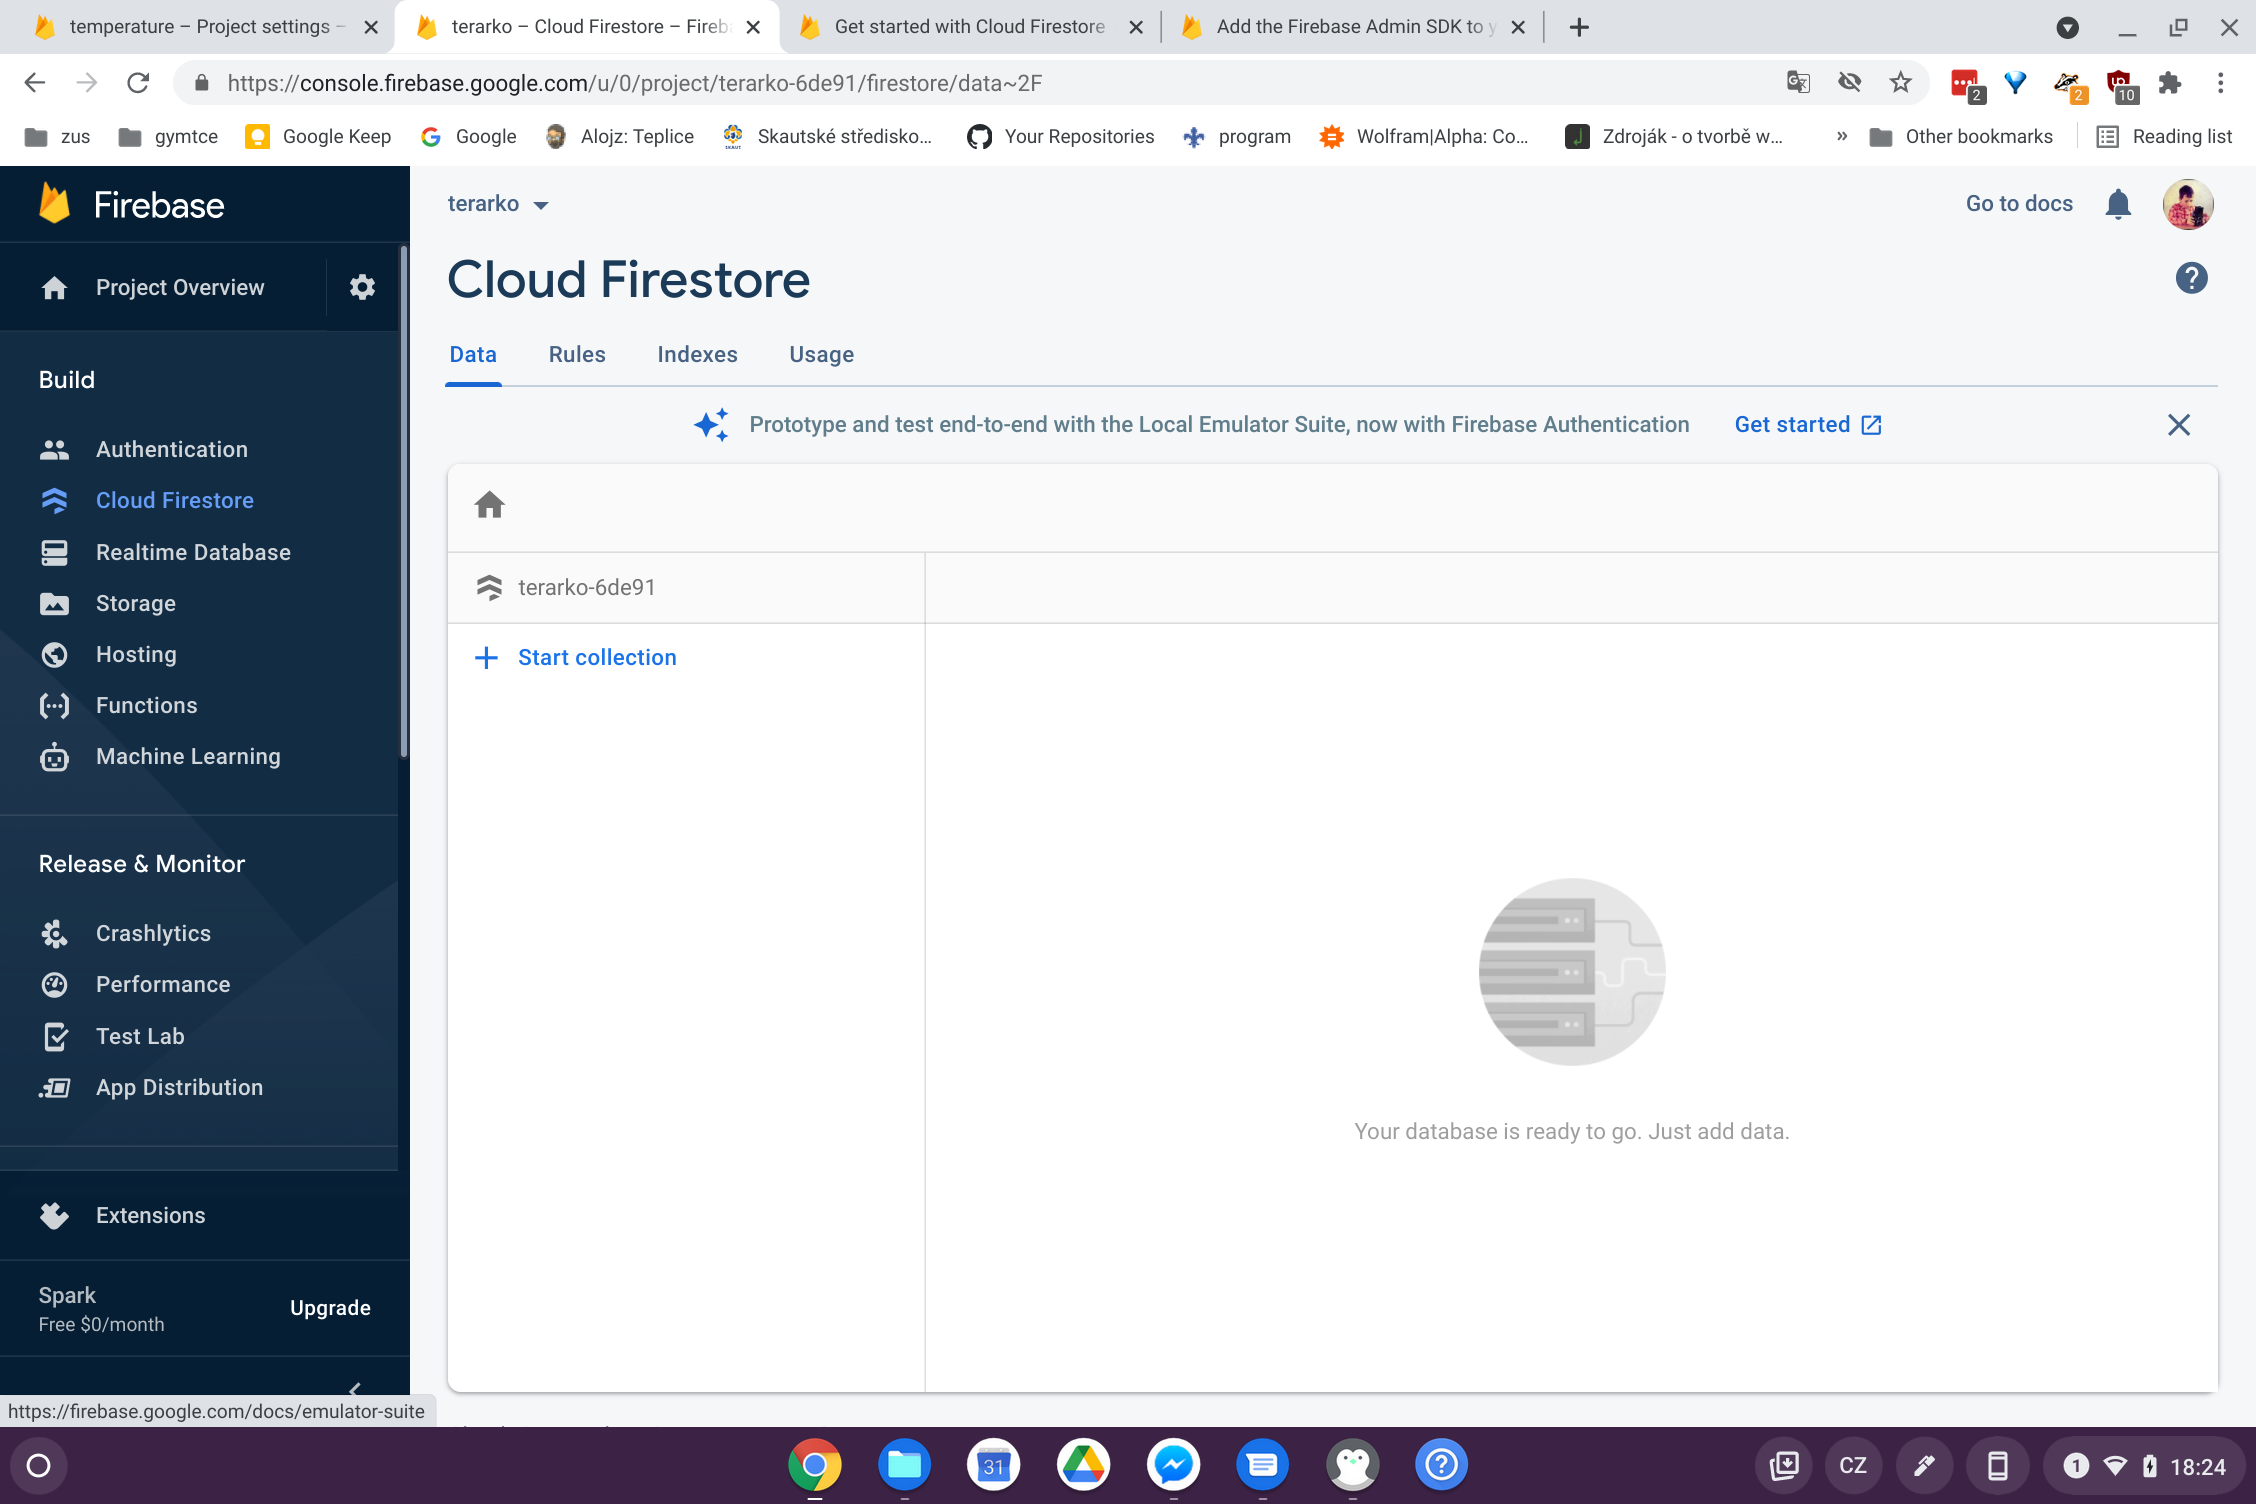
\includegraphics[width=0.8\textwidth]{firestore-dashboard.png}
    \caption{Firestore}
\end{figure}
A mám nastaveno. Teď můžu začít přidávat data.

\subsection{Hosting}
Pro \gls{hosting} jsem použil též platformu \gls{firebase}. Při založení jsem postupoval podle návodu 
(\url{https://firebase.google.com/docs/hosting}). Během inicializace jsem zvolil, že chci pouze \gls{hosting}, pro 
projekt terárko a povolil jsem \gls{github} Actions. Takže po každém commitu, který pošlu na \gls{github} se mi 
automaticky nasadí nejnovější verze stránky. Kvůli tomu jsem zdrojové kódy umístil do samostatného repozitáře.

\subsection{Webová aplikace}
Poslední co je třeba nastavit je samotná webová aplikace a její propojení s \glslink{hosting}{hostingem}. Opět znázorním 
několika obrázky.

% přidání aplikace
\begin{figure}[H]
    \centering
    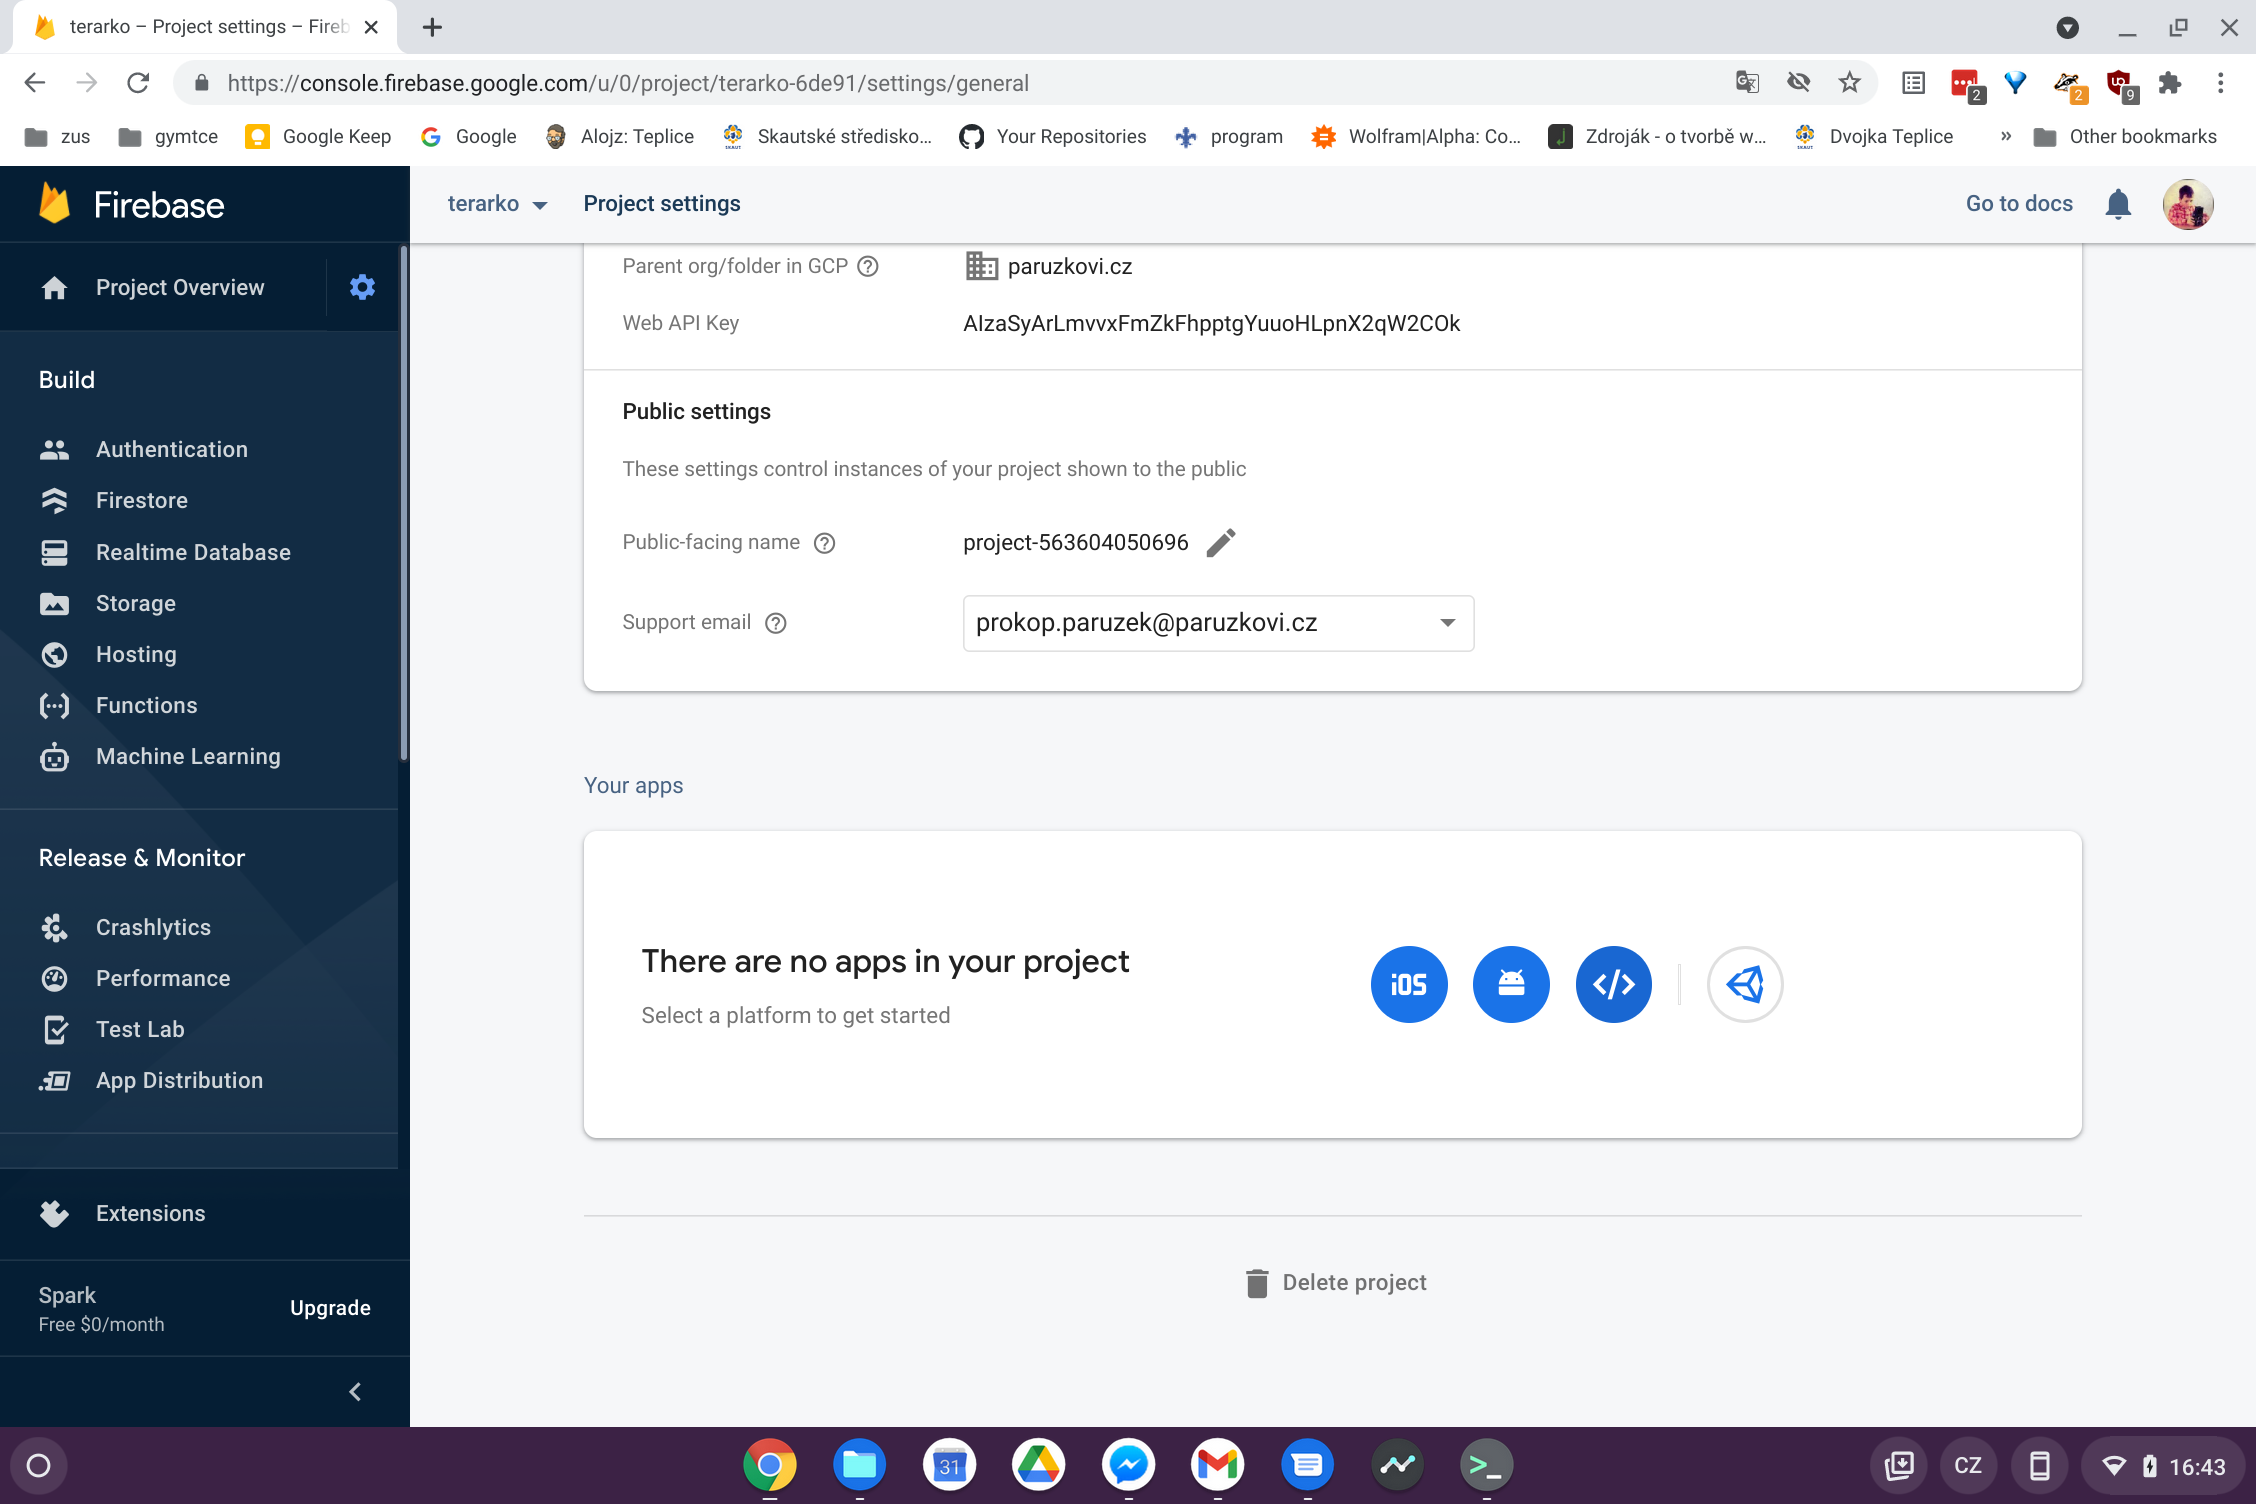
\includegraphics[width=0.8\textwidth]{firebase-addApp.png}
    \caption{Přidání aplikace}
\end{figure}
Přidávám webovou aplikaci, tj. špičaté závorky s lomítkem.
% jméno
\begin{figure}[H]
    \centering
    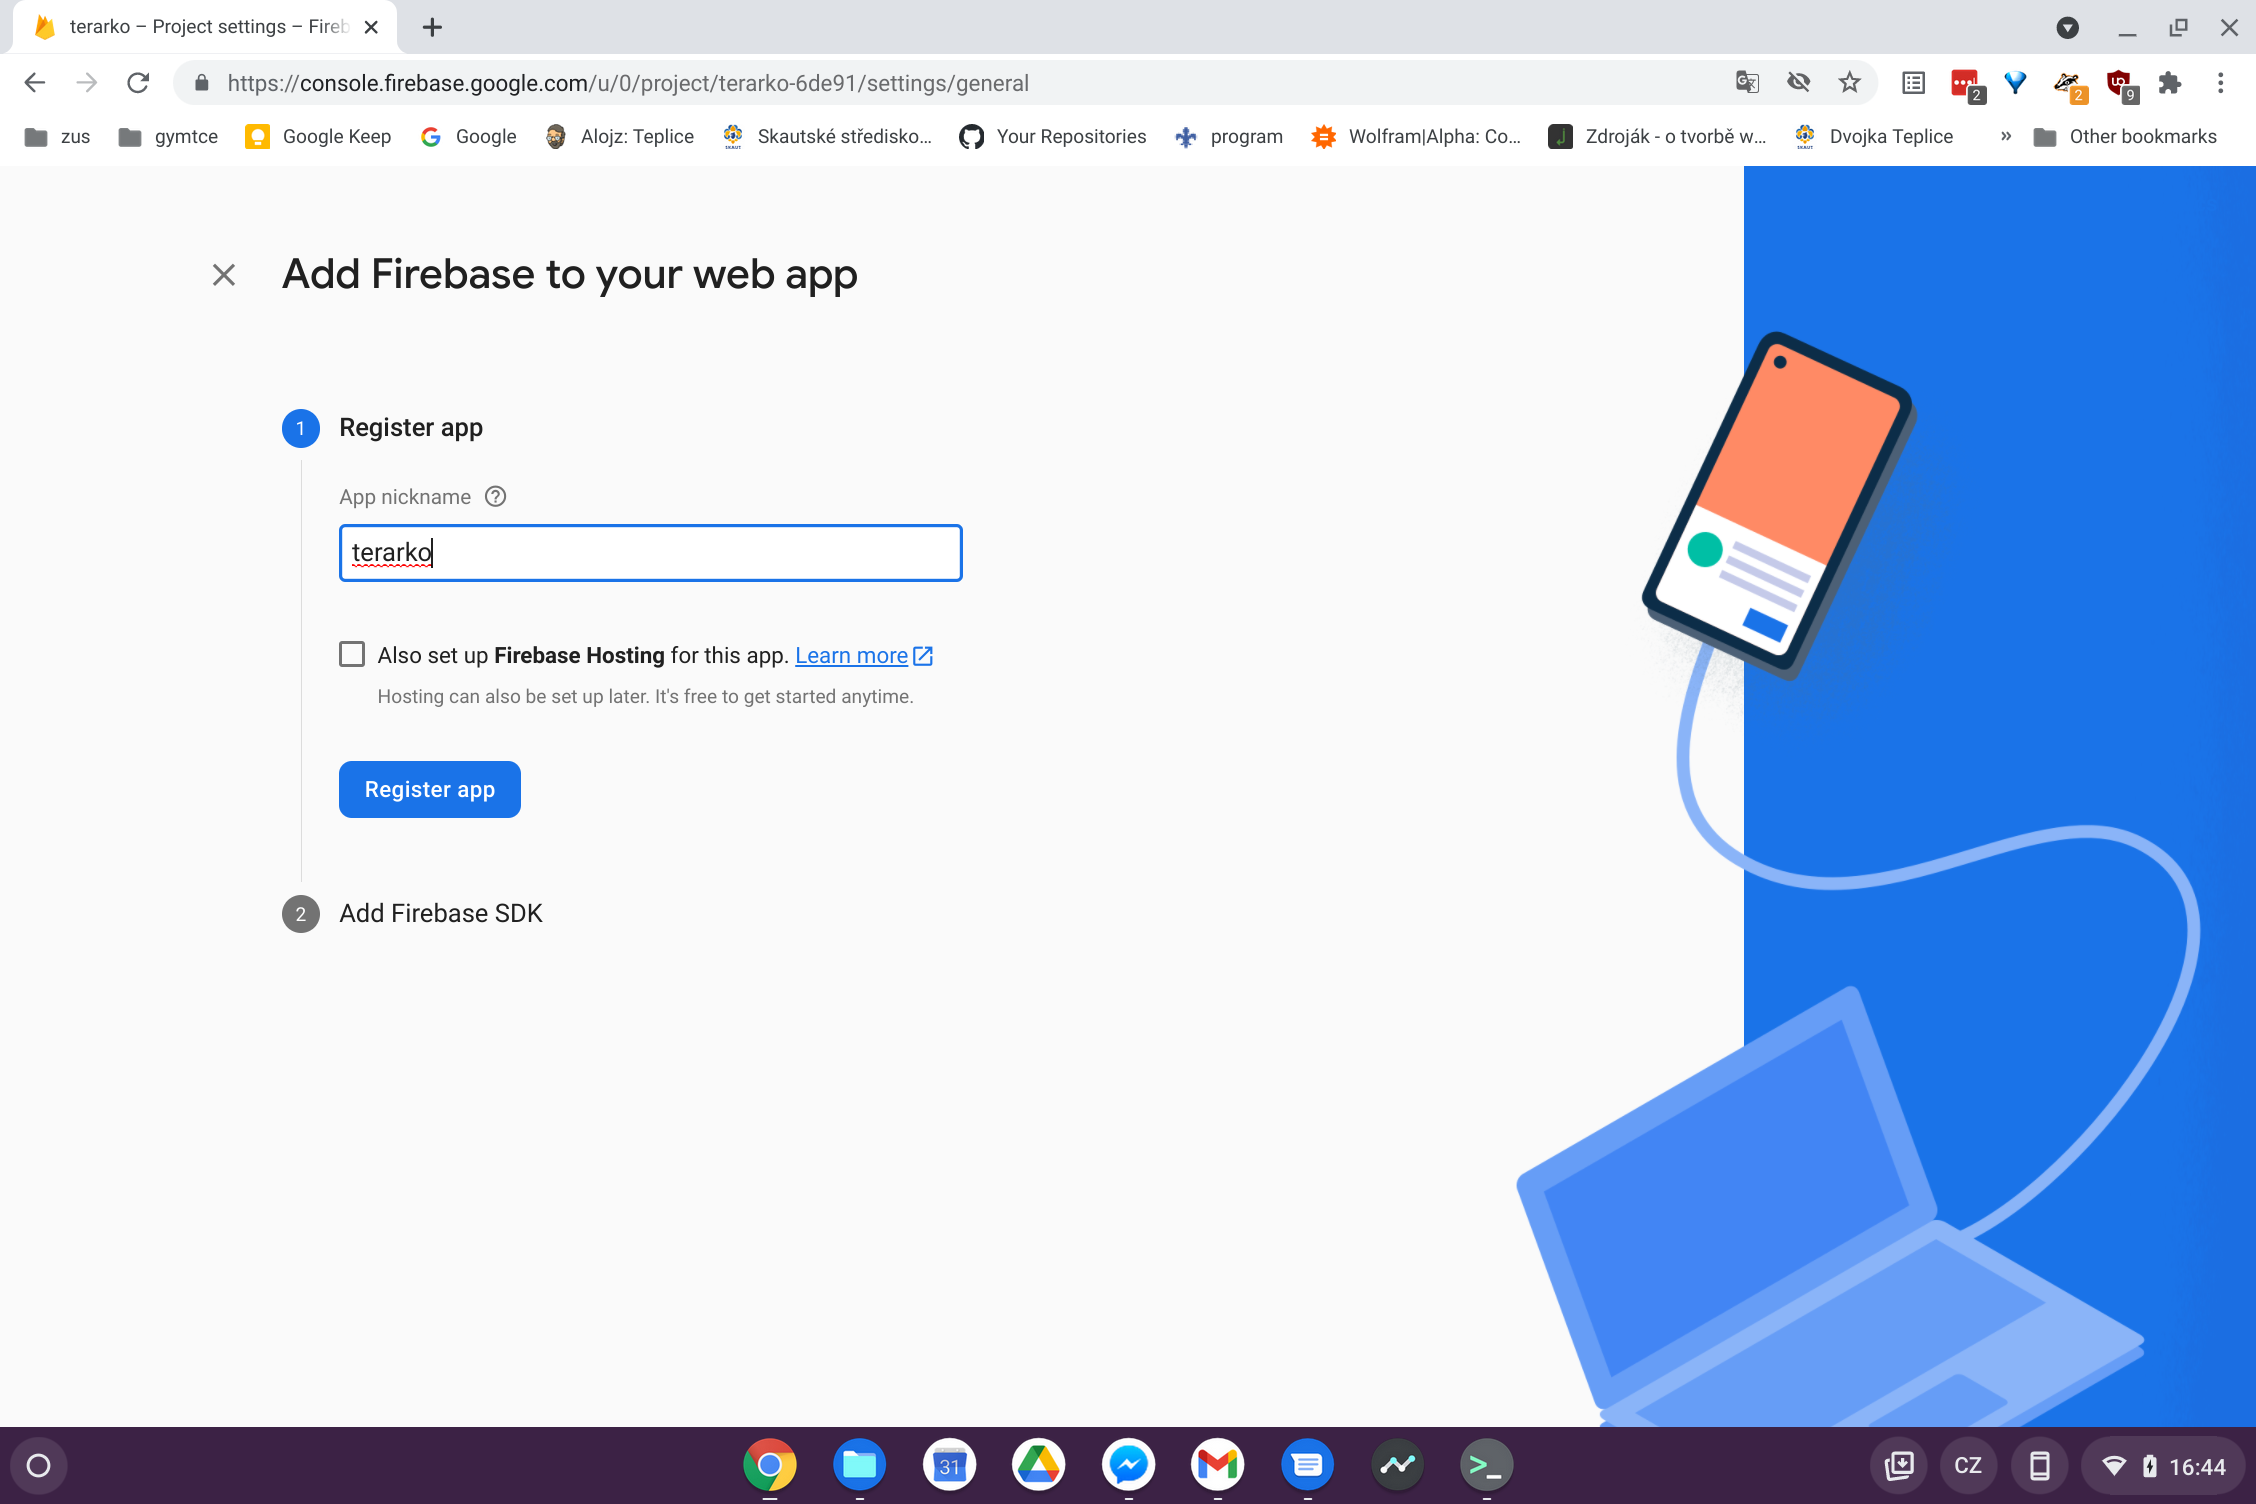
\includegraphics[width=0.8\textwidth]{firebase-app-1.png}
    \caption{Jméno aplikace}
\end{figure}
% SDK
\begin{figure}[H]
    \centering
    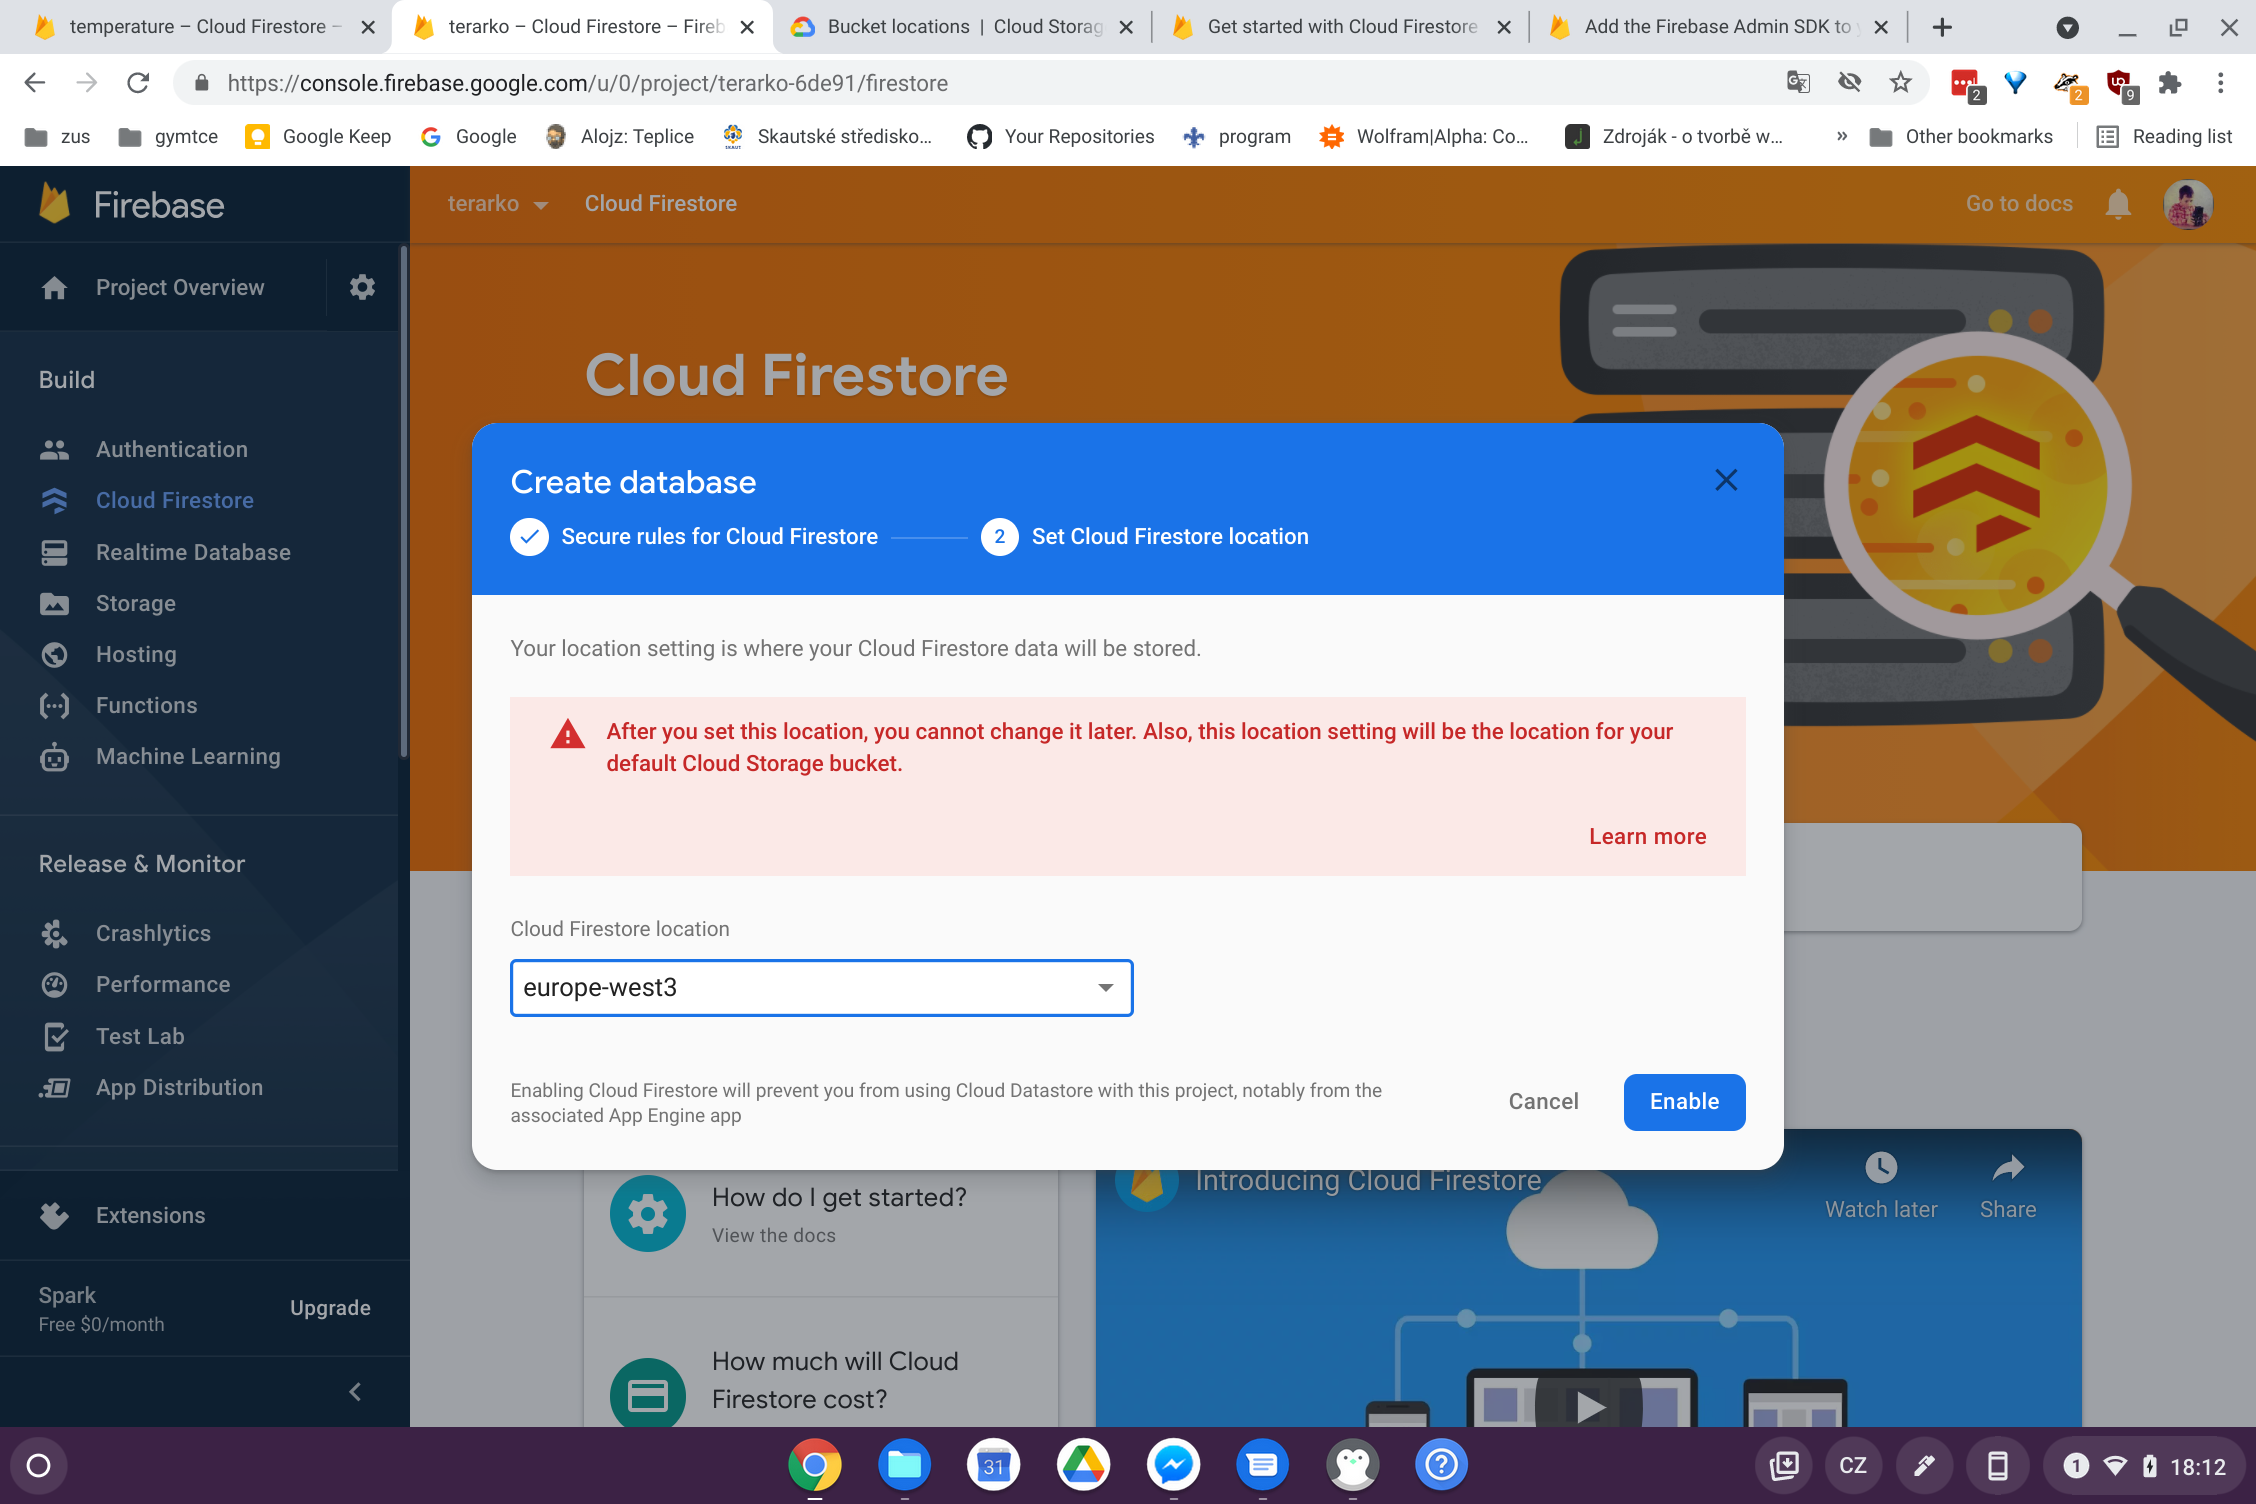
\includegraphics[width=0.8\textwidth]{firestore-2.png}
    \caption{Firestore SDK}
\end{figure}
Toto je důležité pokud si aplikaci hostujete někde u sebe. Já použiji \gls{firebase} \gls{hosting} a tudíž mi to stačí 
odkliknout.
% propojení hostingu
\begin{figure}[H]
    \centering
    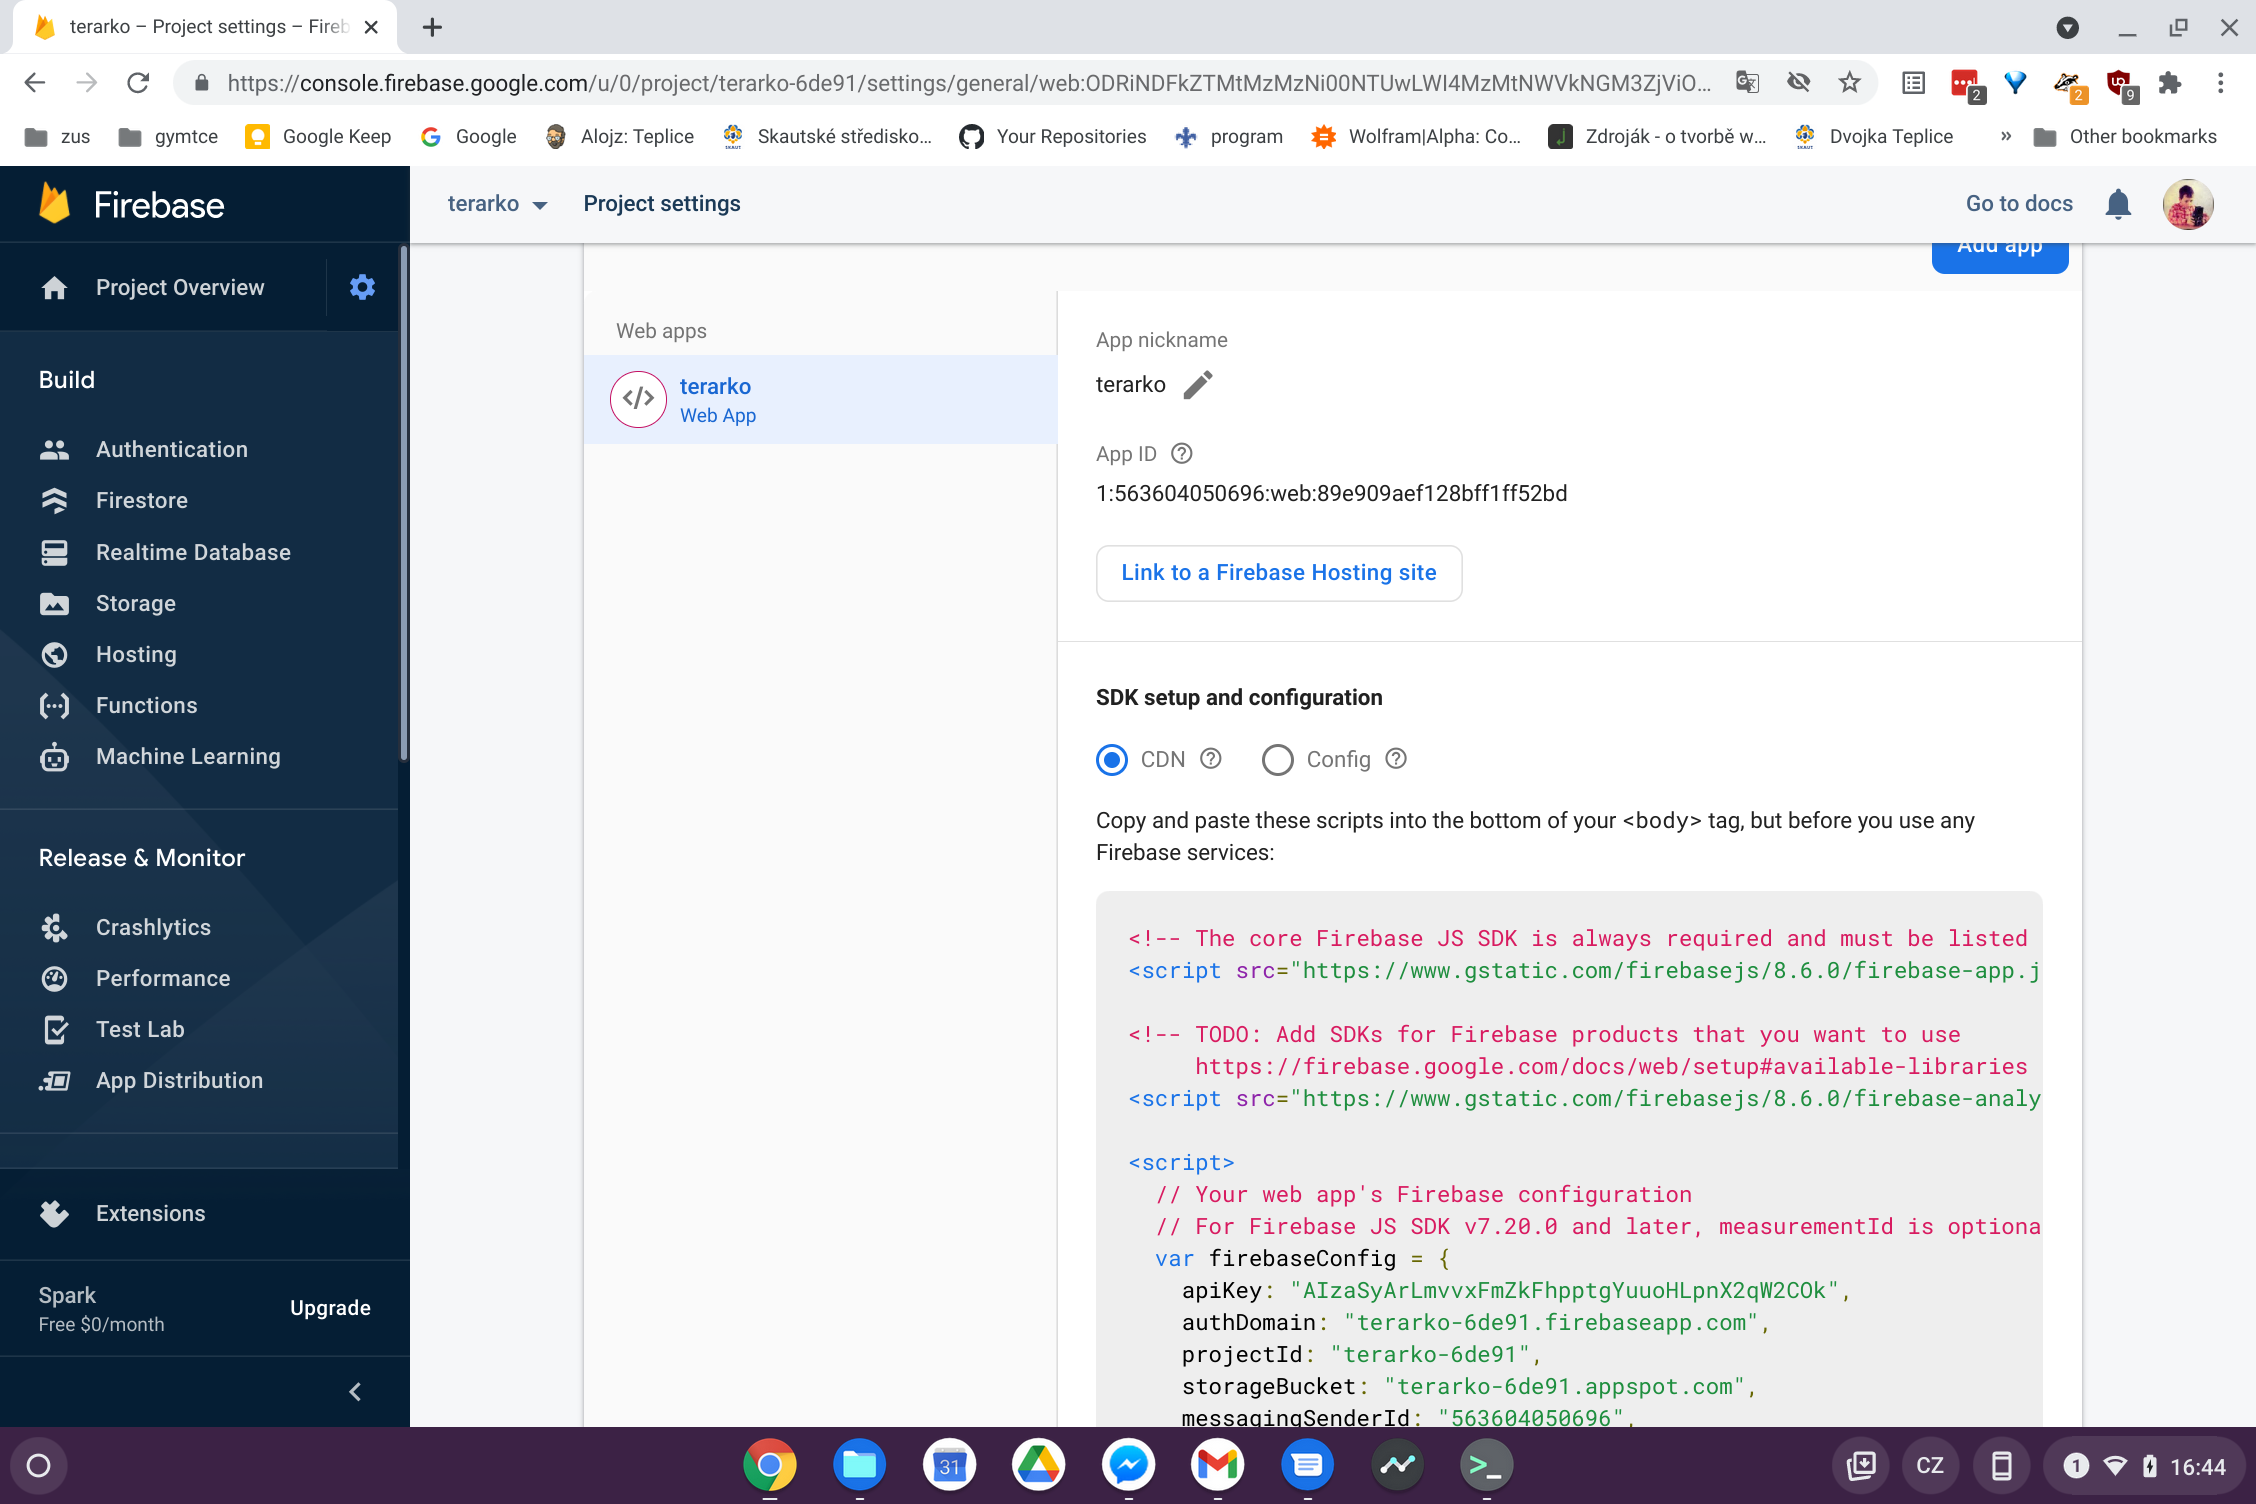
\includegraphics[width=0.8\textwidth]{firebase-app-hosting-1.png}
    \caption{Propojení s hostingem}
\end{figure}
Nyní chci propojit aplikaci s firebase \glslink{hosting}{hostingu}.
% vybrání hostingu
\begin{figure}[H]
    \centering
    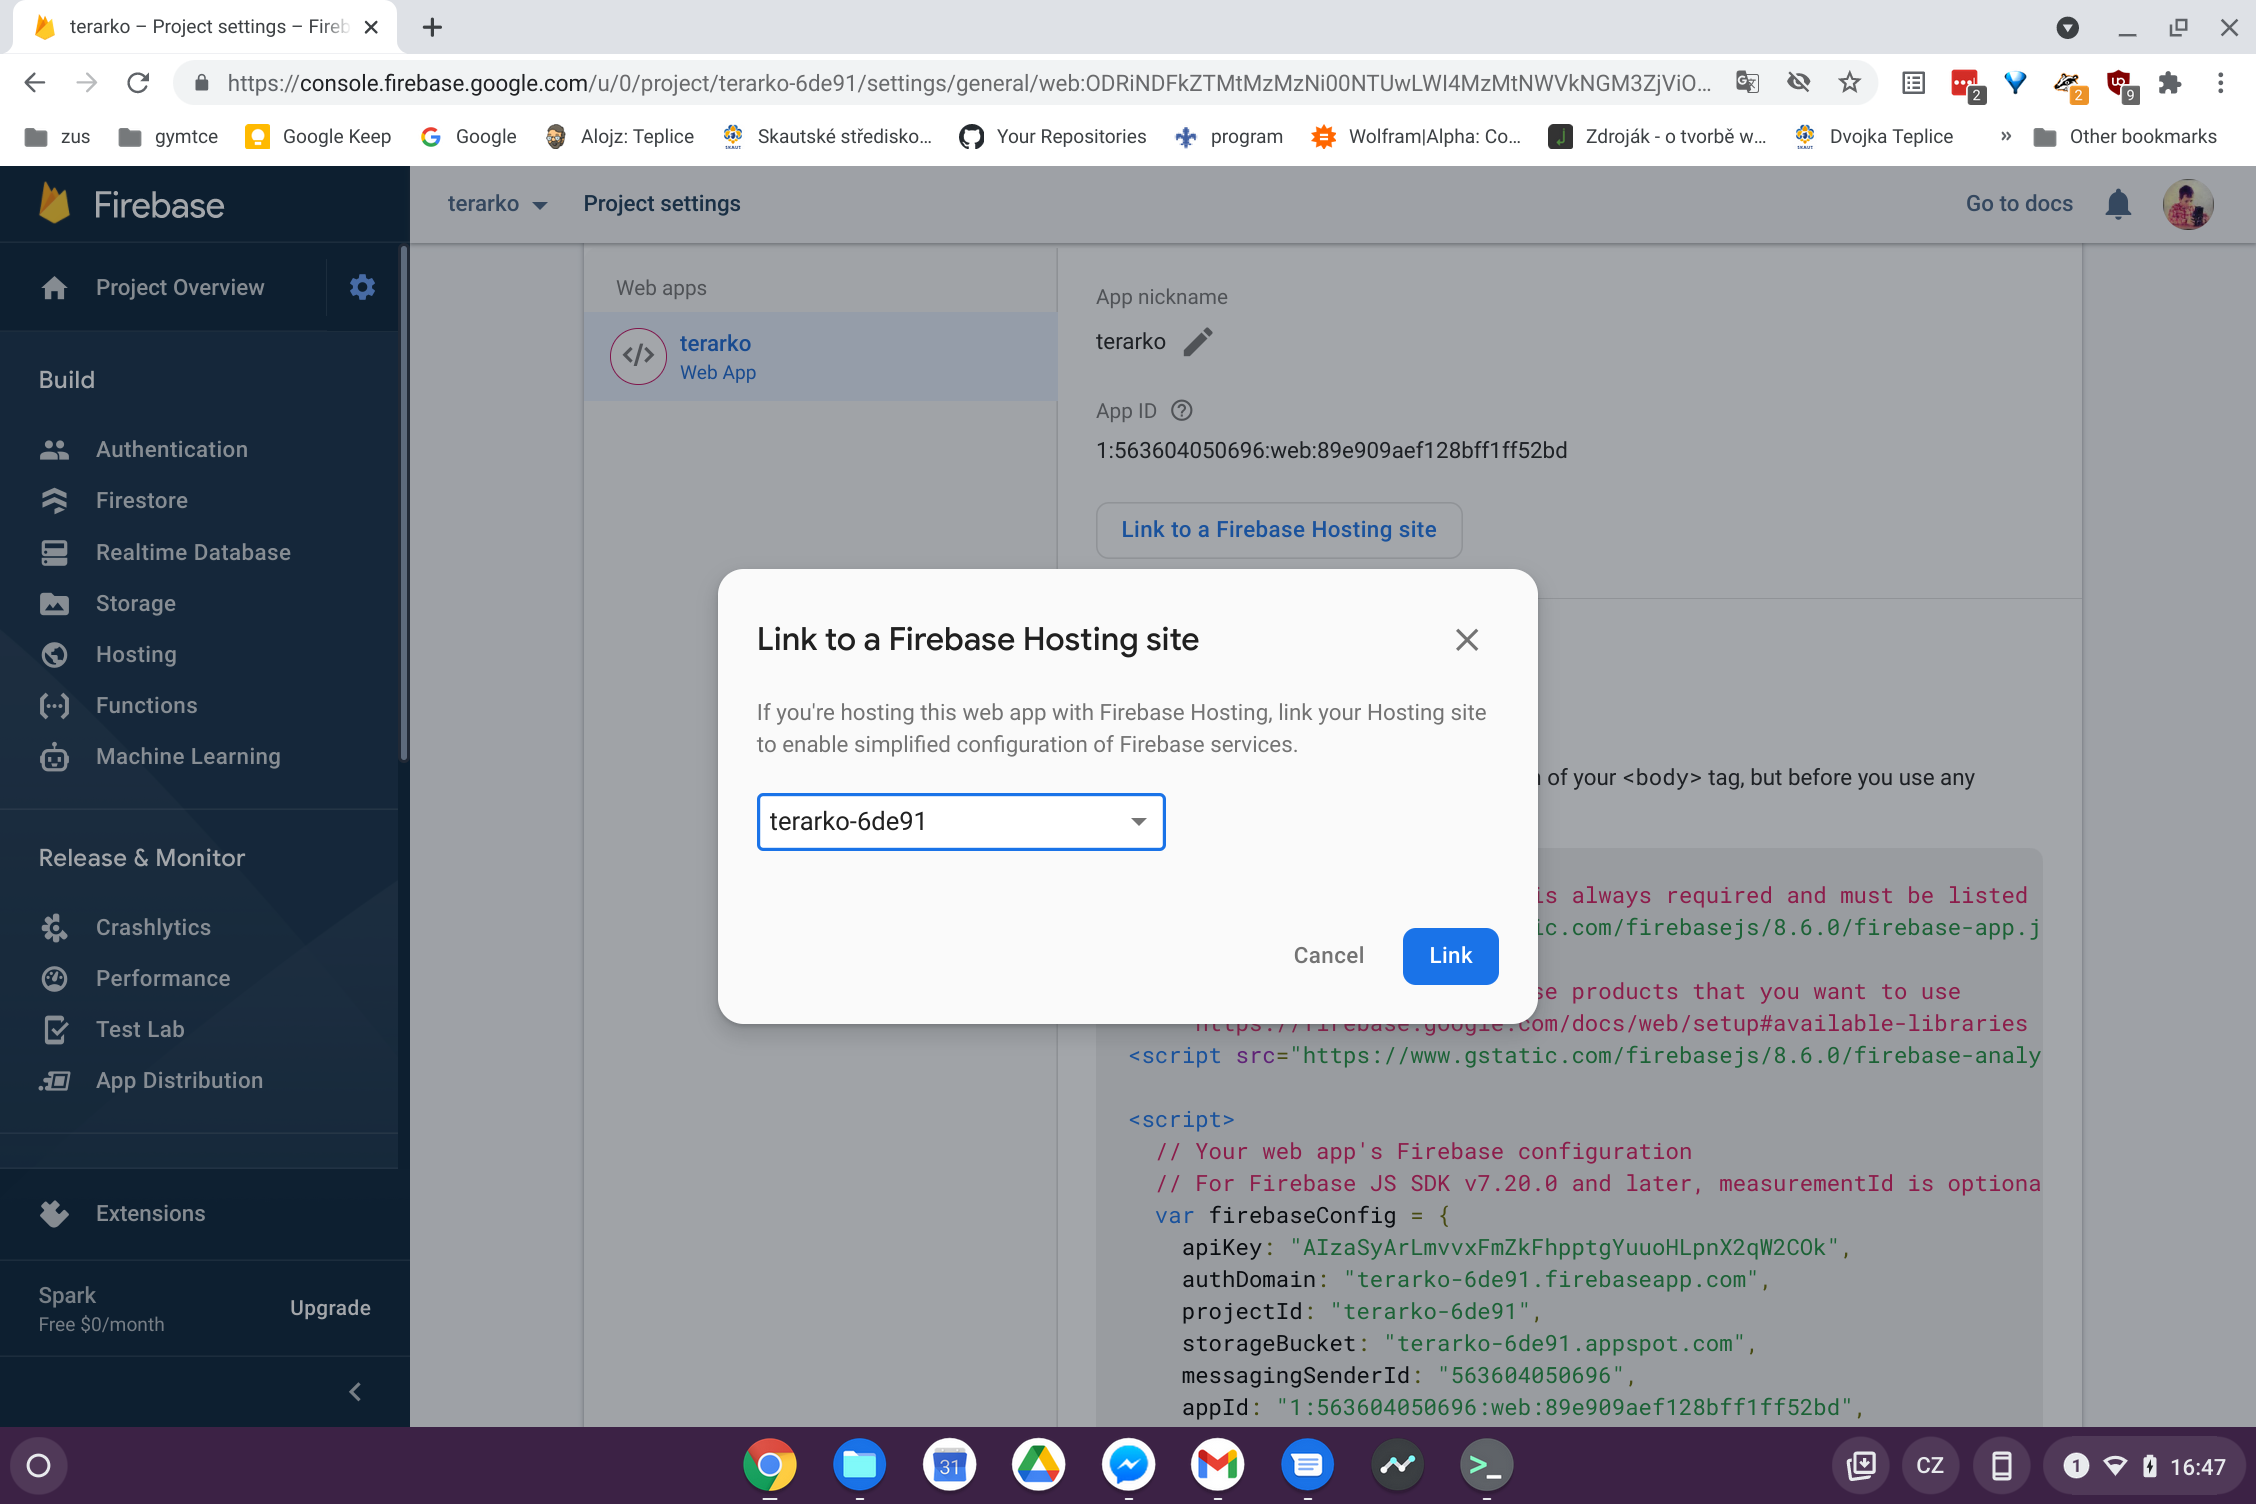
\includegraphics[width=0.8\textwidth]{firebase-app-hosting-2.png}
    \caption{Vybrání hostingu}
\end{figure}
Zde vyberu jaký \gls{hosting} chci použít a to mi umožní zjednodušit kód stránek, protože si všechny ty konfigurační 
údaje načte přímo z \glslink{hosting}{hostingu} spolu s \gls{firebase} \glslink{knihovna}{knihovnami}.
\begin{figure}[H]
    \centering
    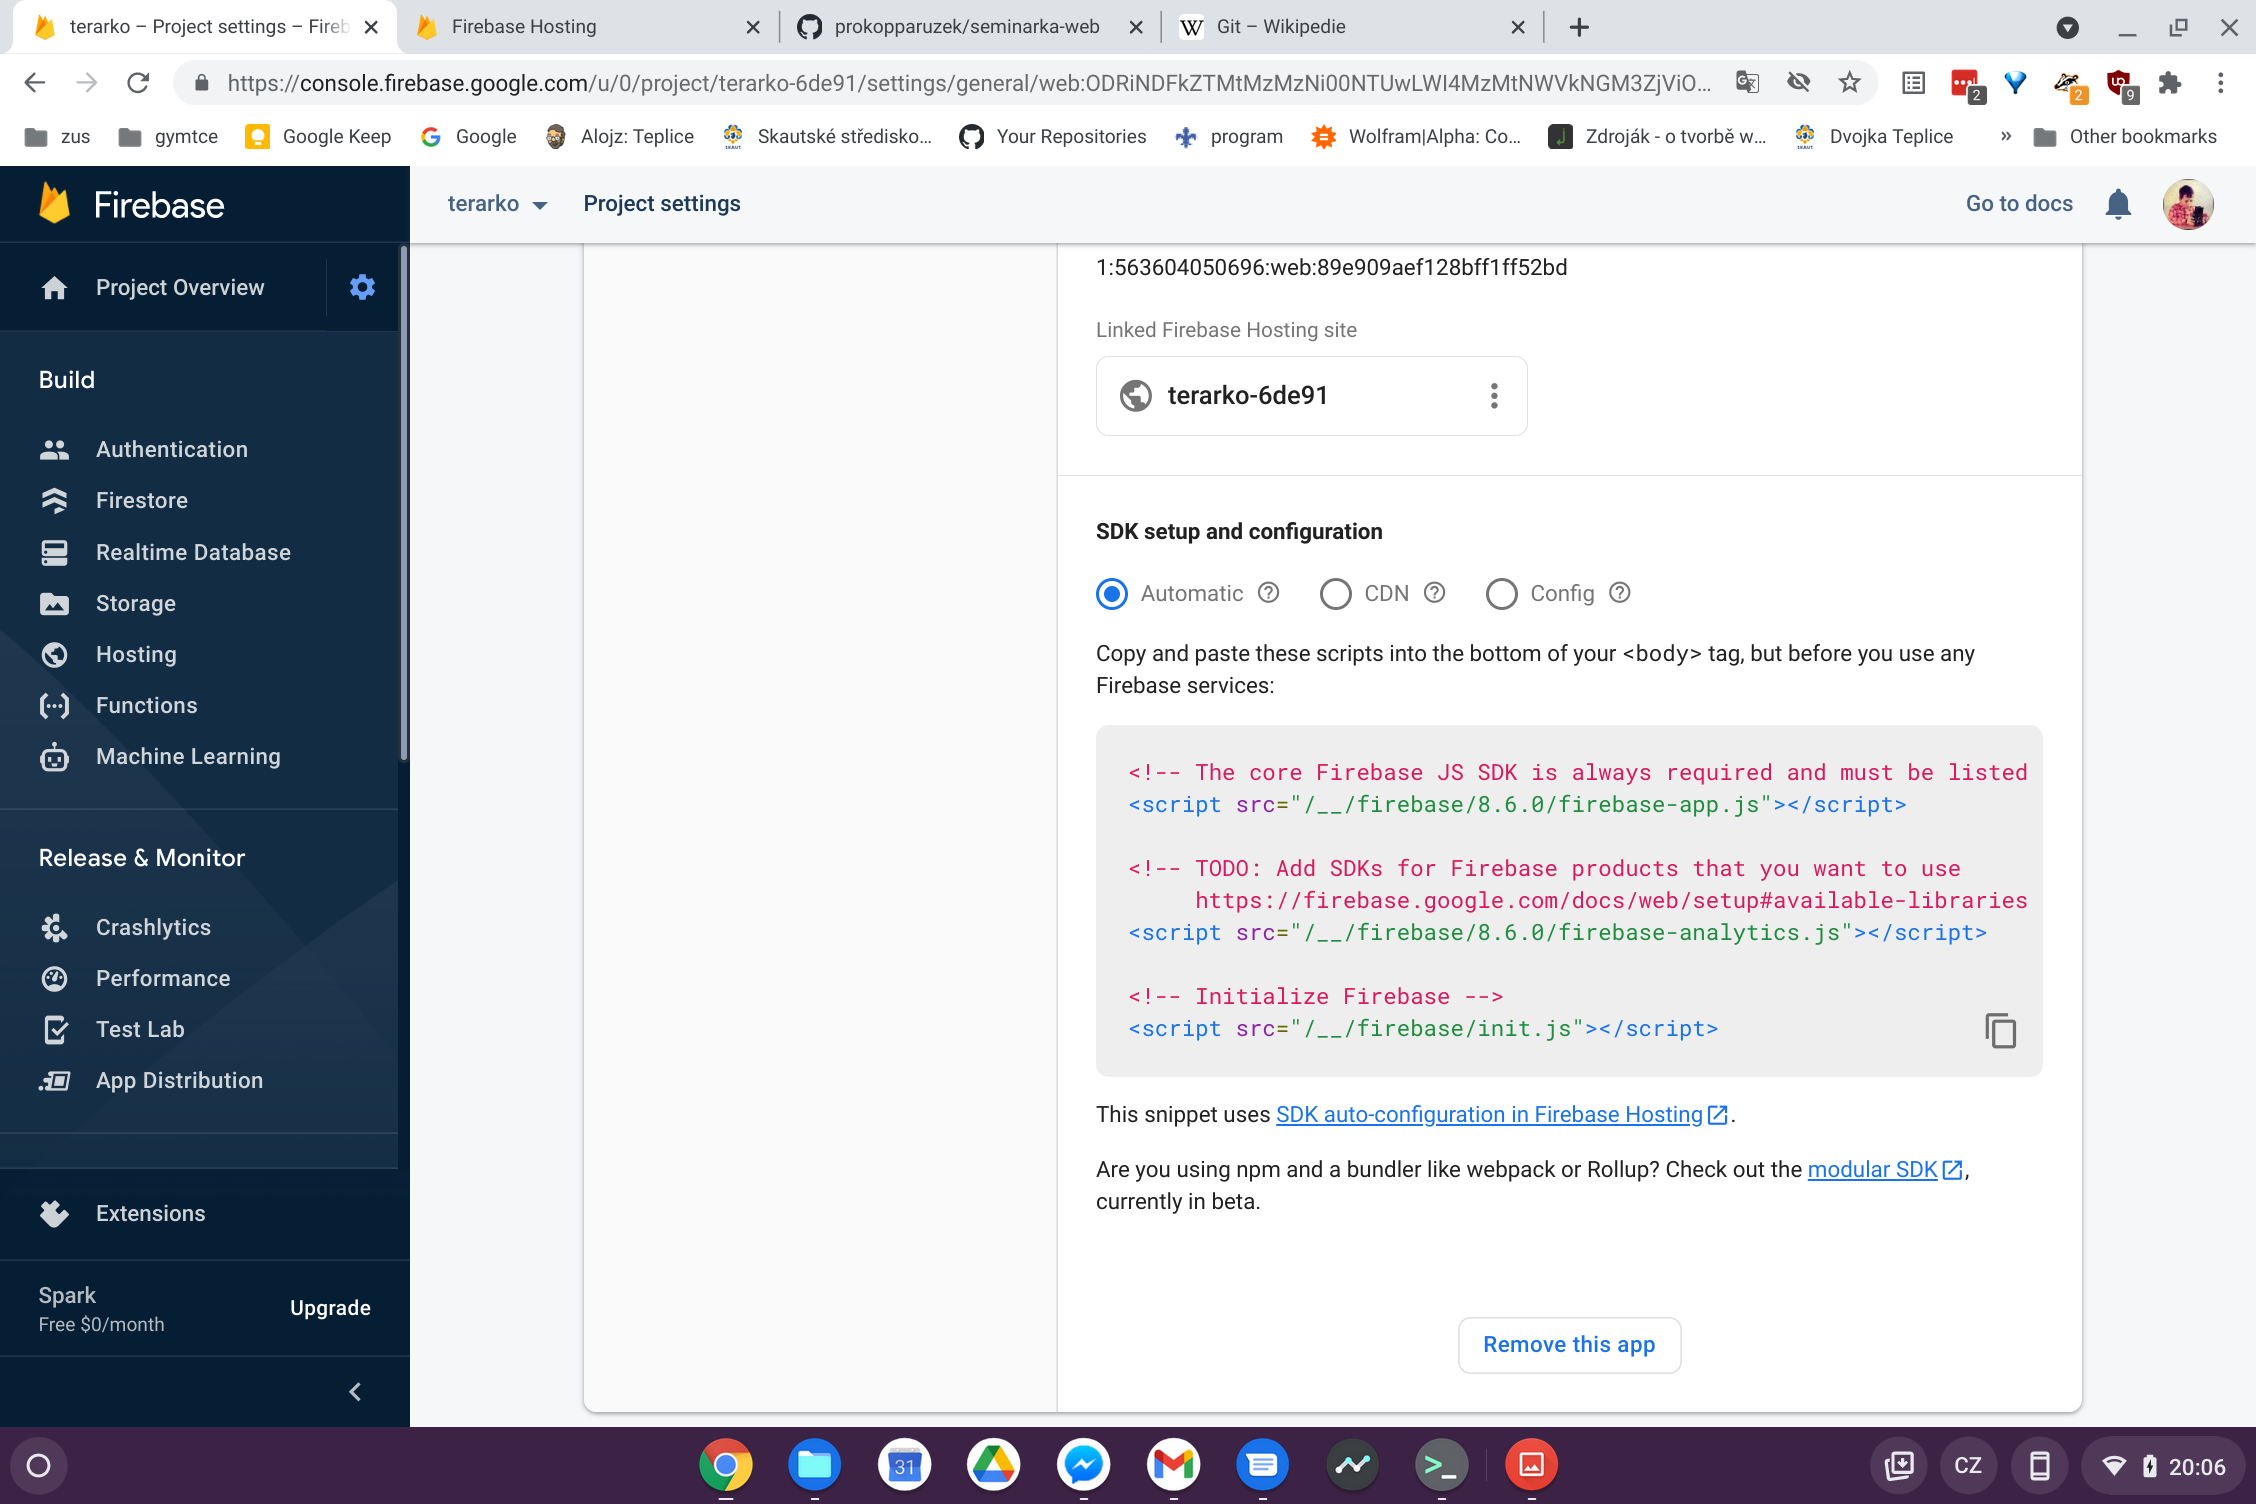
\includegraphics[width=0.8\textwidth]{firebase-app-hosting-3.png}
    \caption{Zjednodušený kód}
\end{figure}
Zde je vidět jak z mnoha řádků kódu zbyly pouze tři při využití \gls{firebase} \glslink{hosting}{hostingu}.
